\RequirePackage{ifluatex}
\let\ifluatex\relax

\documentclass[aps,%
12pt,%
final,%
oneside,
onecolumn,%
musixtex, %
superscriptaddress,%
centertags]{article} %% 
\topmargin=-40pt
\textheight=650pt
\usepackage[english,russian]{babel}
\usepackage[utf8]{inputenc}
%всякие настройки по желанию%
\usepackage[colorlinks=true,linkcolor=black,unicode=true]{hyperref}
\usepackage{euscript}
\usepackage{supertabular}
\usepackage[pdftex]{graphicx}
\usepackage{amsthm,amssymb, amsmath}
\usepackage{textcomp}
\usepackage[noend]{algorithmic}
\usepackage[ruled]{algorithm}
\usepackage{lipsum}
\usepackage{indentfirst}
\usepackage{babel}
\usepackage{pgfplots}
\usepackage{setspace}
\linespread{1.2}
\pgfplotsset{compat=1.9}
\selectlanguage{russian}
\pgfplotsset{model/.style = {blue, samples = 100}}
\pgfplotsset{experiment/.style = {red}}
\theoremstyle{plain}
\binoppenalty=10000
\newtheorem{theorem}{Теорема}[section] %
\setlength{\parindent}{2.4em}
\setlength{\parskip}{0.1em}
%\renewcommand{\baselinestretch}{1.0}
\theoremstyle{definition}
\newtheorem{definition}{Определение}[subsection]
\theoremstyle{remark}
\newtheorem{remark}{Замечание}[section]

\newtheorem{corollary}{Следствие}
\newtheorem{proposition}{Proposition}
\newtheorem{example}{Пример}
\renewcommand*{\proofname}{Proof}

\newtheorem{lemma}{Лемма}[section]

\graphicspath{ {./image/} }
\usepackage{xcolor}
\usepackage{hyperref}


\begin{document}

\begin{titlepage} 
\begin{center}
% Upper part of the page
%\textbf{\Large САНКТ-ПЕТЕРБУРГСКИЙ ГОСУДАРСТВЕННЫЙ ЭКОНОМИЧЕСКИЙ УНИВЕРСИТЕТ} \\[1.0cm]
%\textbf{\large Кафедра Прикладной Математики и Информатики}\\[3.5cm]
 
% Title
\textbf{}\\[10.0cm]
\textbf{\LARGE Билеты по эконометрике}\\[0.5cm]
\textbf{\Large Широков Александр ПМ-1701} \\[0.2cm]

%supervisor
\begin{center} \large
{Преподаватель:} \\[0.5cm]
\textsc {Курышева Светлана Владимировна}\\
\end{center}
\vfill 

% Bottom of the page
{\large {Санкт-Петербург}} \par
{\large {2020 г., 6 семестр}}
\end{center} 
\end{titlepage}

% Table of contents
\begin{thebibliography}{3}
\bibitem{eliseeva}
Эконометрика: Учебник/И.И.Елисеева и др.-М.:Проспект, 2009
\bibitem{praktikuma}
Практикум по эконометрике: Учебное пособие/И.И.Елисеева и др.,М.:Финансы и статистика,2006 
\bibitem{dop1}
Эконометрика: Учебник/В. С.Мхитарян и др.-М.:2008
\bibitem{dop2}
Доугерти К. Введение в эконометрику: Учебник. 2-е изд. / Пер. с англ. – М.: ИНФРА – М, 2007
\bibitem{dop3}
Берндт Э. Практика эконометрики: классика и современность. М.,2005
\end{thebibliography}
\tableofcontents
\newpage


\section{Парная линейная регрессия}

\subsection{Понятие эконометрики. Её место в общественных науках}

\begin{definition}
	\textit{Эконометрика} - это наука, которая дает конкректное количественное выражение закономерностям и взаимосвязям экономических явлений и процессов с помощью статистико-математических методов и моделей.
\end{definition}

\textbf{Связь эконометрики с другими науками:}

\begin{itemize} 
  \item Экономическая теория (сущность связи явлений)
  \item Статистика (информационная база)
  \item Математические и статистические методы:
  \begin{itemize} 
  	\item $C=k\cdot Y+L$, $0<|k|<1$ - регрессия
  	\item $r=sC+Dx+T$, где $t$ - сбережения, а $x$ - инвестиции
  	\item Если s=D, то $t=s(C+x)+T$  - уравнение двухфакторной регрессии
  	\item $Y+r=C+x$ - балансовое тождество 
  \end{itemize} 
\end{itemize}
\newpage
\subsection{Этапы проведения эконометрического исследования }

В качестве этапов эконометрического исследования можно указать:
\begin{enumerate}
	\item Теоретическое описание рассматриваемого процесса
	\item Сбор данных, анализ их качества
	\item Спецификация модели
	\begin{enumerate}
		\item Выявление объясняемых ($Y$) и объясняющих ($X$) переменных 
		\item Выбор функций
	\end{enumerate}
	\item Оценка параметров модели
	\item Верификация модели (т.е проверка достоверности)
	\item Интерпертация результатов 
\end{enumerate}

Данный список включает в себя те стадии, которые проходит любое исследование, независимо от того, на исопльзование каких данных оно ориентировано.
\newpage
\subsection{Спецификация модели. Её суть и назначение}

В эконометрике широко используются методы статистики, эконометрика прежде всего связана с методами регрессии и корреляции.

В зависимости от количества факторов, включенных в уравнение регрессии, принято различать парную и множественную регрессию.

\begin{definition}
	\textit{Парная регрессия} - модель, где среднее значение объясняемой переменной $y$ рассматривается как функция одной независимой (объясняющей) переменной $x$, то есть это модель вида:
	$$\hat{y} = f(x)$$
\end{definition}

\begin{definition}
	\textit{Множественная регрессия} представляет собой модель, где среднее значение объясняемой переменной $y$ рассматривается как функция нескольких независимыъ переменных $x_1,x_2,\ldots$, то есть это модель вида:
	$$\hat{y} = f(x_1,x_2,\ldots,x_k)$$
\end{definition}

Любое эконометрическое исследование начинается с \textit{спецификации модели}, то есть с формулировки вида модели исходя из соответствующей теории связи между переменными.

1. Из всего круга факторов нужно выбрать \textit{наиболее существенное} влияющие факторы. Парная регрессия достаточна, если имеется доминирующий фактор, который и используется в качестве объясняющей переменной.

\begin{definition}
	\textit{Случайная величина} $\xi$ - влияние неучтенных в модели факторов, случайных ошибок и особенностей измерения. Ее присутствие обусловлено спецификацией модели, выборочным характером исходных данных, особенностями измерения переменных.
\end{definition}

\textit{К ошибкам спецификации} будет относиться не только неправильный выбор той или иной математической функции, но и недоучёт в уравнении регресии какого-либо существенного фактора, а также могут иметь место ошибки выборки.

Наибольшую опасность в практическом использовании методов регрессии представляют \textit{ошибки измерения}, на основании которых все время на эксперимент может быть потрачено зря.

Предполагая, что ошибки измерения сведены к минимуму, основное внимание в эконометрических исследоваиях уделяется \textit{ошибкам спецификации модели}.

В парной регрессии спецификация модели связана с выбором математической функции, а в множественной - также с отбором факторов, включаемых в модель.

2. В парной регресси выбор вида математической функции $\hat{y_x} = f(x)$ может проводиться тремя способами:
\begin{itemize}
	\item Аналитический
	\item Графический
	\item Экспериментальный
\end{itemize}

3. Класс математических функций для описания связи двух переменных достаточно широк. Наиболее употребляемыми в модели парной регрессии являются:
$$y=ax+b,\qquad y=a+\frac{b}{x},\qquad y=a+bx+cx^2$$
$$y=ax^b, \qquad a=b^x, \qquad y=ae^{bx} $$

4. Если уравнение регрессии проходит через все точки корреляционного поля, что возможно только при функциональной связи, то фактические значения признака совпадают с теоретическими, то есть они \textit{полностью обсуловлены влиянием фактора $x$}. В этом случае остаточная дисперсия равна $0$.

В практических исследованях имеет место некоторое рассеяние точек относительно линии регрессии. Оно обусловлено влиянием прочих не учитываемых в регресии факторов. 

Иными словами, имеет место отклонения фактических данных от теоретических $y - \widehat{y}_x$.

Чем меньше величина остаточной дисперсии, тем в меньшей мере наблюдается влияние прочих неучитываемых в уравнении регресии факторов и тем лучше уравнение регрессии подходит к исходным данным.

5. Результаты исследований говорят, что число наблюдений должно в $6-7$ раз превышать число рассчитываемых параметров.
\newpage
\subsection{Методы, используемые в эконометрических исследованиях}

1. Для проведения правильных связей нужно знать всю совкупность связей между переменными. Одним из первых методов к решению задчаи явился \textit{метод конфлюэтного анализа}, который предложил изучать целую иерархию регрессий между всеми сочетаниями переменных. Этот метод позволил сделать вывод о наличии какого-то оптимального круга переменных.

На основе изменения коэффициентов регрессии и множественного коэффициента детерминации переменные были разделены на \textit{полезные, лишние и вредные}. Переменная считалась полезной, если ее включение повышало $R^2$ значительно, если добавлялась, не изменяя коэффициентов, то она являлась лишней, если изменяла коэффициенты, то вредной.

2. \textit{Методы корреляций и регрессий} создавались как методы опиания совместных изменений двух и более переменных. 

3. Потребонсть в причнном объяснении корреляции привелка Райта к созданию \textit{метода путевого анализа}. Каждый коэффициент парной корреляции рассматривается как мера полной связи двух переменных.

4. Для определения параметров тенда может использоваться \textit{метод наимеьших квадратов}.

Эконометрический метод складывался в преодолении следующих неприятностей, искажающих результаты применения классических статистических методов:

\begin{itemize}
	\item мультиколлинеарности объясняющих переменных
	\item эффекты гетероскедастичности - отсутствие нормального распределения остатков для регрессионной функции
	\item автокорреляция
	\item ложная корреляция
	\item наличие лагов
\end{itemize}

Последовательность анализа регрессии
\begin{enumerate}
	\item Выбор типа математической функции при построении уравнения регрессии
	\item Оценка параметров уравнения
	\item Показатели силы связи
	\item Статистическая оценка достоверности ($F$-критерий Фишера)
	\item Интвервальная оценка параметров уравнений парной регрессии
	\item Использование модели
\end{enumerate}
\newpage
\subsection{Оценка параметров моделей регрессии}

Рассмотрим случаи, для которых мы хотим предпооложить, что одна \textit{зависимая} переменная $Y$ определяется другими переменными, называемые \textit{объясняющими} переменными (регрессорами). Математическая зависимость, связывающая эти переменные, называется \textit{моделью регрессии}. Мы допускаем, что модель регрессии имеет факт неточности - \textit{случайный} (остаточный) член.

Начнем с рассмотрения простешей модели:
$$ Y_i = \alpha + \beta X_i + \xi_i \eqno (1) $$

$Y_i$ - значение зависимой переменной, $\alpha$ и $\beta$ - постоянные величины - параметры уравнения, $\xi_i$ - случайный член.

Задача регрессионого анализа состоит в получении оценок $\alpha$ и $\beta$ и, следовательно, в определении положения прямой по точкам $\Leftrightarrow$ нужно посроить прямую, в наибольшей степени соответствующую этим точкам.

$a$ - отсечение $Y$ - оценка $\alpha$

$b$ - угловой коэффициент  - оценка $\beta$

\begin{definition}
	Параметр $b$ называется \textit{коэффициентом регрессии}. Его величина показывает \textit{среднее изменение результат} с изменением фактора на единицу.
\end{definition}

Знак $b$ показывает направление связи: при $b>0$ - связь прямая, при $b<0$ - связь обратная.

Интерпретировать при $a$ можно лишь знак. Если $a>0$, то относительное изменение результат происходит медленее, чем изменение фактора. Иными словами, вариация результата меньше вариации фактора.

Пусть $$\widehat{Y} = a+bX_i \eqno (2)$$ 
оцениваемая модель, а $Y_i$ - оцененное значение $Y$. Наша задача заключается в том, чтобы выяснить, существут ли способы оценки коэффициентов $a,b$ алгебраическим путем.

Обозначим за $$e_i = Y_i - \widehat{Y_i} =Y_i - a - bX_i \eqno (3)$$

Остаток наблюдений зависит от выбора коэффициентов $a$ и $b$ $\Rightarrow$ задача заключается в том, чтобы выбрать такие $a$ и $b$, предсказанное значение функции от искомой в каждой точке было минимальным. Глупо минимизировать сумма остатков, потому что при выборе выборочного среднего модели: $$\sum e_i = 0 \eqno (4)$$ 

Поэтому будем минимизировать сумму квадратов остатков. Данный метод называется \textit{Методом Наименьших Квадратов} или сокращенно МНК.
\subsubsection{Предпосылки МНК и их учёт при построении уравнения регрессии}

Условия, необходимые для получения несмещеных, состоятельных и эффективных оценок, представляют собой предпосылки МНК, соблюдение которых желательно для получения достоверности результатов.

Делаются предположения относительно поведения остатков $\xi_i$.

1. Модель линейна по параметрам

2. $\mathbb{E}\xi_i = 0 \forall i$, т.е ожидание значения случайного члена должно быть равно нулю в каждом наблюдении из-за того, что каждое наблюдение не должно включать в себя смещения ни в каком из направлений.

3. Гомоскедастичность - $\mathbb{D}\xi_i = Const $, т.е его значение в каждом наблюдении получено из распределения с постоянной теоретической дисперсией. Также не должно быть причин , делающих его больше подверженным ошибке в одних наблюдениях по сравнению с другим. Заметим, что $$\mathbb{E}\xi_i^2 = \mathbb{D}\xi_i = \mathbb{D}\sigma_{\xi_i}^2 | \forall i $$

4. Отсутствие автокорреляции остатков - значения случайного члена имеют взаимно независимые распределения. Случайный член не подвержен автокорреляции, т.е отсутствует систематическая связь между его значениями в любых двух наблюдениях.
Ковариация равна нулю:
$$ \sigma_{\xi_{i}\xi_{j}} = \mathbb{E}(\xi_i\xi_j) = \mathbb{E}\xi_i \cdot \mathbb{E}\xi_j = 0 | \forall i \neq j $$

5. $\xi_i \sim \mathbb{N}(0,\sigma^2)$: если случайный член нормально распределен, то распределены нормально и коэффициенты регрессии.

После построения уравнения регрессиии проводится проверка наличия у оценок $\xi_i$ тех свойств, которые предполагались. Связано это с тем, что оценки параметров регресии должны отвечать определенным критериям: быть несмещенными, состоятельными эффективными.

\begin{definition}
	Оценка является \textit{несмещенной}, если математическое ожидание остатков равно нулю.
\end{definition}

Следовательно, остатки не будут накапливаться и найденный параметр регрессии $b_i$ можно рассматривать как среднее значение из возможного большого количества несмещенных оценок.

\begin{definition}
	Оценки называются \textit{эффективными}, если они характеризуются наименьшей дисперсией.
\end{definition}

Это означает возможность перехода от точечного оценивания к интервальному.

\begin{definition}
	Состоятельность оценок характеризует увеличение их точности с увеличением объема выборки.
\end{definition}

При соблюдении введенных предпосылок, оценки, полученные методом наименьших квадратов, обладают данными важнейшими свойствами, на основании которых можно быть уверенным в достоверности результатов модели.

\subsubsection {Метод наименьших квадратов}

Пусть у нас имеются $n$ наблюдений $(X_i,Y_i)$, $Y$ зависит от $X$ и мы хотим подобрать уравнение: $$\widehat{Y} = a+bX_i$$

Запишем формально нашу задачу в обозначениях метода наименьших квадратов (МНК):

$$ S = \sum (Y_i-\widehat{Y_i})^2 = \sum (Y_i - a - bX_i)^2 \to min \eqno (5) $$
$$\left\{
\begin{matrix}
\frac{\partial S }{\partial a} = -2 \sum Y + 2na+2b\sum X = 0 \\[0.3cm]

\frac{\partial S }{\partial b} = -2 \sum YX + 2a\sum X+2b\sum X^2 = 0 
\end{matrix} \right. \eqno (6)$$

Применение метода наименьших квадрато приводит к системе уравнений, которая для линейных уравнений имеет вид: \\
$$ \left\{
\begin{matrix}
\sum Y = na + b\sum X \\[0.3cm]
\sum YX = a\sum X + b\sum X^2 \\
\end{matrix} \right. \eqno (7) $$

Решим данную систему линенйных уравнений методом Крамера:
$$ \delta =
\begin{vmatrix}
n & \sum X \\
\sum X & \sum X^2\\
\end{vmatrix}
= n\cdot \sum X^2 - (\sum X)^2 $$

$$ \delta_{b} =
\begin{vmatrix}
n & \sum Y \\
\sum X & \sum XY\\
\end{vmatrix} = n\cdot \sum XY - \sum X\sum Y $$
$$ b = \frac{\delta_{b}}{\delta} = \frac{n\cdot \sum XY - \sum X\sum Y}{n\cdot \sum X^2 - (\sum X)^2} = \frac{ \frac{\sum XY}{n} -\frac {\sum X\sum Y}{n}}{\frac{\sum X^2}{n} - \frac{(\sum X)^2}{n^2}} = \frac {\overline{XY} - \overline{X} \cdot \overline{Y}}{\overline{X^2} - (\overline{X})^2} = \frac {cov(x,y)}{\sigma_x^2} $$

Итого получаем коэффициенты предполагаемой модели:
$$ b = \frac {cov(x,y)}{\sigma_x^2}  = \frac{\sum (X_i - \overline{X})\cdot (Y_i - \overline{Y})}{\sum (X_i-\overline{X})^2} = \frac {\overline{XY} - \overline{X} \cdot \overline{Y}}{\overline{X^2} - (\overline{X})^2} \eqno (8) $$
$$ a = \overline{Y} - b\overline{X} \eqno (9) $$

$b$ - наклон линии регресии (коэффициент регрессии) - абсолютный показатель силы связи.

Свойства метода МНК (результаты относительно регрессий, оцениваемых по обычному МНК):

\begin{enumerate}
	\item $\sum e_i = 0$
	\item $\overline{e} = 0$
	\item $ \overline{\widehat{Y}} = \overline{Y}$
	\item $\sum X_i \cdot e_i = 0$
	\item $\sum \widehat{Y_i} \cdot e_i = 0$
\end{enumerate}

Парное уравнение регрессии может быть записано в матричной форме:
$$Y = BX + E$$
где 

$Y$ - вектор столбец $n \times 1$ фактических значений результативного признака;

$B$ - вектор столбец размерности $2 \times 1$, подлежащих оценке параметров модели;

$X = (x_0,x_1)$ - матрица размерности $n \times 2$ значений факторов. При этом $x_0=1$ и связано это с наличием в уравнении регрессии свободного члена, а $x_1$ - собственно реальные значения включенного в уравнение регрессии фактора;

$E$ - вектор столбец случайной веичины $\xi_i$ размерности $n \times 1$.

Матрица исходных данных примет вид:
$$Y = \begin{bmatrix}
	y_1 \\ y_2 \\ \vdots \\ y_n
\end{bmatrix}, \qquad X = \begin{bmatrix}
	1 & x_1 \\ 1 & x_2 \\ \vdots \\ 1 & x_n
\end{bmatrix}, \qquad B = \begin{bmatrix}
	a \\ b
\end{bmatrix}, \qquad E = \begin{bmatrix}
	\xi_1 \\ \xi_2 \\ \vdots \\ \xi_n
\end{bmatrix}$$
В матричной форме применение МНК записыватся так:
$$S = (Y-XB)^T (Y-XB) \to \min$$
$$\frac{\partial S}{\partial B} = -2X^TY + 2X^TXB =0$$
$$(X^TX)B = X^TY \Longrightarrow B = (X^TX)^{-1}X^TY$$
\newpage
\subsection{Корреляция, её смысл и значение. Показатели корреляции}

Уравнение регрессии всегда дополняется обязательным показателем тесноты связи. При использовании линейной регресии в качестве такого показателя выступает \textit{линеный коэффициент корреляции $r_{xy}$}.
Существует разные модификации формулы линейного коэффициента корреляции:
$$
r_{xy} = b \frac{\sigma_x}{\sigma_y} =\frac{cov(x,y)}{\sigma_x^2} \cdot \frac{\sigma_x}{\sigma_y} =  \frac{\overline{YX} - \overline{Y} \cdot \overline{X}}{\sigma_x \sigma_y}, -1 \leq r_{xy} \leq 1 \eqno (10)
$$

Если коэффициент регрессии $b>0$, то $0 \leq r_{xy} \leq 1$, если $b<0$, то $-1 \leq r_{xy} \leq 0$.

Следует иметь ввиду, что величина линейного коэффициента корреляции оценивает тесноту связи рассматриваемых признаков в её линейной форме. Поэтому близость абсолютной величины линейного коэффициента корреляции к нулю \textit{еще не означает отсутствие связи} между признаками. При иной спецификации модели связь между признаками модет оказаться достаточно тесной.

Шкала значений коэффициента корреляции (все значения берутся по модулю):
\begin{itemize}
	\item $r_{yx} \leq0.3$ - связь слабая
	\item $0.3 < r_{yx} \leq 0.5$ - связь умеренная
	\item $0.5 < r_{yx} \leq 0.7$ - связь заметная
	\item $0.7 < r_{yx} \leq 0.9$ - связь высокая
	\item $0.9 < r_{yx} \leq 1$ - связь весьма высокая, близкая к функциональной
\end{itemize}

Для оценки качества подбора линейной функции расчитывается квадрат линейного коэффициента корреляции $r_{yx}^2$, называемый \textbf{коэффициентом детерминации}. Коэффициент детерминации характеризует долю дисперсии результативного признака $y$, объясняемую регрессией, в общей дисперсии результативного признака.
$$r_{yx}^2 = \frac{\sigma_{y,obyasn}^2}{\sigma_{y,obch}^2} \eqno (11)$$

Чем больше доля объясненной вариации, тем соответственно меньше роль прочих факторов и, следовательно, линейная модель хорошо аппроксимирует исходные данные и ею можно воспользоваться для прогноза значений результативного признака.

Коэффицинеты регрессии именованные, поэтому несравнимы для разных признаков. 

Линейный коэффициент корреляции как измеритель линейной связи признаков логически связан не только с коэффициентом регрессии $b$, но и с \textbf{коэффициентом эластичности}, который является \textit{показателм силы связи, выржаенным в процентах}.

При линейной связи признаков $x$ и $y$ \textit{средний коэффициент эластичности} вычисляется по формулам:
$$\text{Э}_{yx} = b \cdot \frac{\bar{x}}{\bar{y}}$$

Несмотря на схожесть показателей, измерителем \textit{тесноты связи} выступает линейный коэффициент корреляции $r_{xy}$, а коэффициент регрессии $b$ и коэффициент эластичности $\text{Э}_{yx}$ - показатели \textit{силы связи}. $b$ - абсолютная мера, так как имеет единицы измерения, а коэффициент эластичности - относительная, так как выражена в процентах.

Несмотря на важность измерителя тесноты связи, используют коэффициент детерминации $r_{yx}^2$, ибо он дает меру влияния фактора на результат, фиксируя и роль ошибок, то есть случайных составляющих в формировании моделируемой переменной.
\newpage
\subsection{Оценка качества регрессионных моделей. Стандартная ошибка линии регрессии}

\subsubsection{Оценка качества регрессионных моделей}

Цель регрессии - объяснение поведения $Y$. В любой выборке $Y$ оказывается низким, а в других - высоким. Разброс значений $Y$ можно описать с помощью суммы квадратов отклонений от выборочного среднего.
$$ \sum (Y - \overline{Y})^2 $$

Все показатели корреляции основаны на правиле сложения дисперсий $\Rightarrow$ можно разложить \textbf{общую сумму квадратов отклонений } переменной $Y$ от среднего значения $\overline{Y}$ на две части - \textbf{"объясненную" } сумму квадратов и \textbf{"необъясненную"}. 
$$\sum (Y - \overline{Y})^2 = \sum (\widehat{Y} - \overline{Y})^2 + \sum (Y - \widehat{Y})^2 \eqno (12)$$

Данное равенство можно переписать как:
$$SS_T = SS_R + SS_E \eqno (13)$$

где: 

$SS_T  = \sum (Y - \overline{Y})^2 $  - общая сумма квадратов отклонений \textit{(total sum of squares)}

$SS_R = \sum (\widehat{Y}-\overline{Y})^2 $ - \textbf{сумма квадратов отклонений, объясненная} регрессией, \textbf{факторная сумма} \textit{(sum of square due to regression)}

$SS_E = \sum (Y - \widehat{Y})^2  = \sum e_i^2 $ - \textbf{остаточная сумма} квадратов отклонений,
\textit{(sum of square due to error)}.

Введем \textbf{коэффициент детерминации}:
$$ R^2 = r^2 = \frac{\sigma_{y,obyasn}^2}{\sigma_{y,obch}^2} = \frac{SS_R}{SS_T} = 1 - \frac{SS_E}{SS_T} = 1 - \frac{\sum (Y - \widehat{Y})^2}{\sum (Y - \overline{Y})^2} $$
$$ R^2 = \frac{\sum (\widehat{Y}-\overline{Y})^2}{\sum (Y - \overline{Y})^2} = 1 - \frac{\sum (Y - \hat{Y})^2}{\sum (Y - \overline{Y})^2} \eqno (14) $$

\textbf{Коэффициент детерминации}- обобщающий показатель оценки качества построенного уравнения регрессии.

Если фактор $x$ не влияет на результат, то линия регрессии параллельна оси ox  и $\bar{y} = \hat{y}$. Тогда вся дисперсия результативного признака обусловлена воздействием прочих факторов и общая сумма квадратов отклонений совпадет с остаточной.

Если же прочие факторы не влияют на результат, то $Y$ связан с $X$ функционально и остаточная сумма квадратов $SS_E = \sum e_i^2 = 0$. В этом случае сумма квадратов отклонений равна объясненной сумме квадратов: $$SS_T = SS_R$$

Поскольку не все точки поля корреляции лежат на линии регрессии, то всегда имеет место их разброс как обусловленный влиянием фактора $X$, т.е регрессией $Y$ по $X$, так и вызванный действием прочих причин(необъясненная вариация). 

Так как  $$ R^2 = 1 - \frac{\sum (Y - \widehat{Y})^2}{\sum (Y - \overline{Y})^2}  = 1 - \frac{SS_E}{SS_T},$$ 

то если $SS_T$ будет больше остаточной суммы квадратов $SS_E$, то уравнение регрессии статистически значимо и фактор $X$ оказывает существенное воздействие на результат $Y$. Это равносильно тому, что коэффициент детерминации $R^2$ будет приближаться к единице.

Любая сумма квадратов отклонений связана с числом степени свободы (\textit{df - degrees of freedom}), т.е числом свободы независимого варьирования признака. Число степеней свободы связано с числом единиц совокупности $n$ и с числом определяемых по ней констант.

При расчете объясненной или факторной суммы квадратов $\sum (\widehat{Y} - \overline{Y})^2$ используются теоретические (расчетные) значения результативного признака $\widehat{Y}$, найденные по линии регресии: $$\widehat{Y} = a+bX_i$$ 

Сумма квадратов отклонений, обусловленных линейной регрессией (следует из формулы линейного коэффициента корреляции): 
\label{SSR}
$$ SS_R = \sum (\widehat{Y_i}-\overline{Y})^2 = b^2 \cdot \sum(X-\overline{X})^2 \eqno (15)$$
\begin{proof}
	так как по формулам (11) и (14):
	$$ r_{yx}^2 = \frac{\sigma_{y,obyasn}^2}{\sigma_{y,obch}^2} = \frac{SS_R}{SS_T}=\frac{\sum (\widehat{Y}-\overline{Y})^2}{\sum (Y - \overline{Y})^2} = b^2 \cdot \frac{\sigma_x^2}{\sigma_y^2}  
	$$
	$$\sum (\widehat{Y}-\overline{Y})^2 = b^2 \cdot \frac{\sigma_x^2}{\sigma_y^2} \cdot \sum (Y - \overline{Y})^2 =b^2 \cdot \frac{\sum (X - \overline{X})^2}{\sum (Y - \overline{Y})^2} \cdot \sum (Y - \overline{Y})^2 = b^2 \cdot \sum (X - \overline{X})^2 
	$$
\end{proof}

Данная сумма квадратов отклонений имеет 1 степень свободы, так как зависит только от одной константы коэффициента регрессии $b$, следовательно: $$df_{SS_R} = 1 $$

Число степеней свободы остаточной суммы квадратов при линейной регрессии: $$df_{SS_E}=n-2$$

Число степеней свободы для общей суммы квадратов определяется числом единиц, и поскольку мы используем среднюю вычисленную по данным выборки, то теряем одну степень свободы, следовательно: $$df_{SS_T} = n-1$$

В случае линейной регрессии получаем следующее равенство: $$ n-1 = 1 + (n-2)$$

В общем случае: $$ df_{SS_T} = df_{SS_R} + df_{SS_E}$$ $$ n-1 = m + ( n - 1 - m) $$ 
$$df_{SS_T}=n-1, df_{SS_R} = m, df_{SS_E} = n-1-m \eqno (16)$$
где $m$ - число параметров переменных.

Разделив каждую сумму квадратов на соответствующее ей число степеней свободы, получим средний квадрат отклонений или \textbf{дисперсию на одну степень свободы}:

$$ MS_R = \frac {SS_R} {df_R} = \frac{\sum (\widehat{Y}-\overline{Y})^2} {m} \eqno (17)$$
$$ MS_E = \frac {SS_E} {df_E} = \frac{\sum (Y - \widehat{Y})^2} {n - 1 - m} \eqno (18)$$
$$ MS_T = \frac {SS_T} {df_T} = \frac{\sum (Y - \overline{Y})^2}{n-1}\eqno (19) $$
где $MS_T$ - общая дисперсия, $MS_E$ - остаточная, $MS_R$ - факторная (объясненная).

\newpage
\subsection{Оценка значимости параметров уравнения парной регрессии}

\subsubsection{Статистическая оценка достоверности регрессионной модели}

После того как найдено уравнение линейной регресии, проводится оценка значимости как уравнения в целом, так и отдельных его параметров. Оценка значимости уравнения регрессии в целом дается с помощью $F$-критерия Фишера. При этом выдвигается нулевая гипотеза, что коэффициент регрессии равен нулю, т.е $b=0$ и, следовательно, фактор $x$ не оказывает влияния на результат $Y$.

Выберем нулевую гипотезу, по которой мы будем оценивать качество модели (в генеральной совокупности):
\begin{center}
	$H_0$: $r^2 = 0 $  \\
	$H_1$: $r^2 \neq 0 $ 
\end{center}

Определение дисперсии на одну степень свободы приводит дисперсии к \textit{сравнимому виду}. Сопоставляя факторную (объясненную) и остаточную дисперсию в расчете на одну степень свободы, получим величину \textbf{$F$-критерия}:
\label{Snedekor}
$$F=\frac {MS_R} {MS_E } =  \frac {\text{Factor Variance with 1 df} } {\text{Remainder variance with 1 df}} \eqno (20)$$

Значение $F_{table}$ означает максимальную величину отношения дисперсия при случайном их расхождении для данного уровня вероятности и наличия нулевой гипотезы.

В математической статистике данное распределение называется распределение \textit{Снедекора} для $(n,m)$ степеней свободы.

Для проверки гипотезы о значимости уравнения регресии воспользуемся следующим алгоритмом:
\begin{enumerate}
	\item Выберем в достоверной области критический уровень значимости $\alpha$. Обычно выбирают маленький уровень значимости, так как вероятность попадания в критическую область при справедливости нулевой гипотезы $H_0$ должна быть маленькой ($\alpha \approx 0.05$).
	\item Определяется табличное критическое значение критерия Фишера $F_{table}(m,n-1-m)$
	\item Если $F>F_{table}$, то $H_0$ отвергается $\Rightarrow$ гипотеза о случайности природы отвергается и делается вывод о существенности связи и значимости $R^2$
\end{enumerate}

Если нулевая гипотеза справедлива, то факторная (объясненная) и остаточная дисперсия не отличаются друг от друга. 
Величиная $F$-критерия связана с коэффициентом детерминации $r^2$. Факторную сумму квадратов отклонений можно представить как:
$$ SS_R = \sum (\widehat{Y_i}-\overline{Y})^2 = b^2 \cdot \sum(X-\overline{X})^2  = r_{yx}^2\cdot \sigma_y^2 \cdot n \eqno (21)$$

так как:
$$ SS_R = \sum (\widehat{Y_i}-\overline{Y})^2 = r_{yx}^2 \cdot SS_T = r_{yx}^2 \sum (Y - \overline{Y})^2 =$$
$$ r_{yx}^2 \cdot \frac{1}{n} \sum (Y - \overline{Y})^2 \cdot n = r_{yx}^2 \cdot \sigma_{y}^2 \cdot n  $$

А остаточную сумму квадратов как:
$$ SS_E = \sum (Y_i-\widehat{Y_i})^2 = (1-r_{yx}^2)\cdot \sigma_y^2 \cdot n \eqno (22)$$

так как:

$$ r_{xy}^2 = 1 - \frac{SS_E}{SS_T} \Rightarrow SS_E = SS_T \cdot (1-r_{xy}^2) = (1-r_{yx}^2)\cdot \sigma_y^2 \cdot n $$

Тогда значение $F$-критерия равно:
\label{FR}
$$F = \frac {MS_R} {MS_E } = \frac{\frac {SS_R} {df_R}}{\frac {SS_E} {df_E}} = \frac{r_{yx}^2}{(1-r_{yx}^2)} \cdot \frac{n-1-m}{m} \eqno (23)$$ 
где $n$ - число единиц в совокупности, $m$ - число параметров при переменных.

Результаты факторного анализа обычно представлены в таблице дисперсионного анализа
\label{first_table_analiz}
\begin{table}[H]
	\begin{center}
		\begin{tabular}[t]{|c|c|c|c|c|} \hline
		Источник вариации & df & $SS$ & $MS$ & F-критерий\\ \hline
		Регрессия & 1 & 14735 & 14735 & 278 \\ \hline
		Остаток & 5 & 265 & 53 & 1 \\ \hline
		Итого & 6 & 15000 & x & x \\ \hline
		\end{tabular}
	\caption{Таблица дисперсионного анализа для примера}
	\end{center}
\end{table}
$F_{table} = 6.61$, 278 > 6.61 - регресия статистически значима, $r^2 \neq 0$

\subsubsection{Оценка значимости коэффициентов регрессии} 

В линейной регресии обычно оценивается значимость не только уравнения в целом, но и отдельных его параметров. С этой целью по каждому из параметров строится его \textbf{стандартная ошибка} (случайная ошибка коэффициента регрессии).

Выдвигается нулевая гипотеза о равенстве коэффициентов регресии в генеральной совокупности:
$$H_0: b= 0 $$ 
$$H_1: b \neq 0 $$ 

\textbf{Стандартная ошибка} коэффициента регрессии определяется по формуле:
$$m_b= \sqrt {\frac{MS_E}{\sum (X-\overline{X})^2}} = \sqrt {\frac{\frac{\sum (Y - \widehat{Y})^2} {n - 1 - m}}{\sum (X-\overline{X})^2}} \eqno (24)$$

Вводится t-статистика:
$$ t_{b}=\frac {b - 0}{m_b} = \frac{b}{m_b} \sim t(n-m-1 =n-2) \eqno (25)$$

так как два параметра, то число степеней свободы равно двум и данная статистика имеет распределение Стьюдента с $n-2$ степенями свободы.

Для проверки гипотезы о значимости коэффициента регресии воспользуемся следующим алгоритмом:
\begin{enumerate}
	\item Выберем в достоверной области критический уровень значимости $\alpha$. Обычно выбирают маленький уровень значимости, так как вероятность попадания в критическую область при справедливости нулевой гипотезы $H_0$ должна быть маленькой. 
	\item Определяется табличное критическое значение критерия Стьюдентая $t_{table}(n-m-1 = n-2)$
	\item Если $|t_{b}| > t_{table}$, то $H_0$ отвергается $\rightarrow$ гипотеза о незначимости коэффициента регрессии отвергается (параметр $b$ не случайно отличается от нуля, и сформировался под влиянием систематически действующего фактора)
\end{enumerate}

Критерий опровержения гипотезы:

\begin{equation*}
	|t_{b}| = \frac {b} {m_b} = \frac {b} {\sqrt {\frac{MS_E}{\sum (X-\overline{X})^2}}} > t_{table} \Leftrightarrow H_o \text { discards} \eqno (26)
\end{equation*} 

Величина $m_b$ называется случайной ошибкой коэффициентов регресии. 
Если $t_b > 3 $, то параметры всегда значимы.

\subsubsection{Связь F и t-критериев}
$F$-критерий Снедекора и $t$-критерия Стюдента для коэффициентов регрессии взаимосвязаны. Покажем эту связь:
$$t_b^2 = \frac{b^2}{m_b^2} = \frac {b^2}{\frac{\frac{\sum (Y - \widehat{Y})^2} {n - 1 - m}}{\sum (X-\overline{X})^2}}  =  \frac {b^2 \cdot {\sum (X-\overline{X})^2}}{\frac{\sum (Y - \widehat{Y})^2} {n - 1 - m}} \stackrel{\ref{SSR}}{=} \frac{SS_R}{\frac{\sum (Y - \widehat{Y})^2} {n - 1 - m}} = \frac{MS_R}{MS_E} = F $$

Следовательно:
\label{svyaz_tb_F}
$$t_b = \sqrt {F} \eqno (27)$$

\newpage
\subsection{Интервальная оценка параметров уравнения линейной регрессии}

Если коэффициенты регрессии оказываются статистически значимыми, то можно построить \textbf{доверительный интервал} для коэффициентов регрессии:
$$\delta_b = \pm t_{table} \cdot {m_b}$$
$$ b - t_{1 - \frac{\alpha}{2}}(n-2) \cdot {m_b} \leq b \leq b + t_{1 - \frac{\alpha}{2}}(n-2) \cdot {m_b} \eqno (35)$$

$\delta_b$ назывют также \textit{предельной ошибкой}.

Также стандартную среднюю ошибку для коэффициента $a$ можно выразить через $m_b$:
$$ m_a = \sqrt{\frac{\sum (Y - \widehat{Y})^2} {n - 1 - m} \cdot \frac{\sum X^2}{n\cdot (X-\overline{X})}} = m_b \cdot \sqrt{\frac{\sum X^2}{n}} \eqno (36)$$

\newpage
\subsection{Прогнозирование по однофакторным моделям регрессии. Стандартная ошибка линии регрессии}

В прогнозных расчетах по уравнению регрессии определяется предсказываемое ($y_p$) значение как точечный прогноз $\widehat{y_x}$ при $x_p=x_k$, т.е путем подстановки в уравнение регрессии $\widehat{y_x} = a+b \cdot x$ соответствующего значения $x$. Однако точечный прогноз явно нереален, поэтому он дополняется расчетом стандартной ошибки $\widehat{y_i}$, т.е $m_{\widehat{y}}$ и соответственно интервальной оценкой прогнозированного значения $y^*$.

Выражение для \textbf{стандартной ошибки предсказываемого по линии регрессии значения} $\widehat{y}$:
$$ m_{\widehat{y_x}} = \sqrt{MS_E} \sqrt{\frac{1}{n}+\frac{(x_k-\overline{X})^2}{\sum(X-\overline{X})^2}} \eqno (37) $$

где $\sqrt{MS_E}$ - корень из остаточной дисперсии на одну степень свободы.
Данная формула стандартной ошибки предсказываемого значения $y$ при заданном значении $x_k$ и характеризует ошибку положения линии регрессии.

Величина стандартной ошибки достигает минимума при $x_k  = \overline{X} $.

Для прогнозируемого значения $\widehat{y}$ доверительный интервал выглядит следующим бразом:
$$ \widehat{y_{x_k}} \pm t_{1-\frac{\alpha}{2}}(n-2) \cdot m_{\widehat{y_x}} $$
$$ \widehat{y_{x_k}} - t_{1-\frac{\alpha}{2}}(n-2) \cdot m_{\widehat{y_x}} \leq \widehat{y_{x_k}} \leq \widehat{y_p} + t_{1-\frac{\alpha}{2}}(n-2) \cdot m_{\widehat{y_x}}  \eqno (38)$$

где:
$$ \widehat{y_{x_k}} = a+b\cdot x_k $$

\textbf{Средняя ошибка прогнозируемого индивидуального значения} составит:
$$ m_y = \sqrt{MS_E} \sqrt{1+\frac{1}{n}+\frac{(x_k-\overline{X})^2}{\sum(X-\overline{X})^2}} \eqno (39)$$

\textbf{Доверительный интервал для $y_p$ }- предсказываемого значения регрессии:
$$ \widehat{y_p} - t_{1-\frac{\alpha}{2}}(n-2) m_y \leq y_p \leq \widehat{y_p} + t_{1-\frac{\alpha}{2}}(n-2) m_y \eqno (40) $$

\newpage
\section{Нелинейная парная регрессия}

\subsection{Нелинейный модели парной регрессии. Общая характеристика}

Если между явлениями существуют нелинейные соотношения, то они выражаются с помощью соответствующих нелинейных функций.

Различают два класса \textit{нелинейной регрессии}:
\begin{enumerate}
	\item Нелинейная по независимым переменным - регрессии, нелинейные относительно включенных в анализ объясняющих переменных, но линейные по оцениваемым параметрам.
	\item Нелинейная по оцениваемым параметрам 
\end{enumerate}

Примеры нелинейной регрессии по независимым переменным:
\begin{enumerate}
	\item полиномы разных степеней: $ y = a + bx + cx^2+ \varepsilon $
	\item равносторонняя гипербола: $ y = a + \frac{b}{x} + \varepsilon $
\end{enumerate}

Примеры нелинейных регрессий по оцениваем параметрам:
\begin{enumerate}
	\item степенная: $ y = a \cdot x^b \cdot \varepsilon $
	\item показательная: $ y = a \cdot b^x \cdot \varepsilon $
	\item экспоненциальная: $ y =e^{a+bx} \cdot \varepsilon $ 
\end{enumerate}

Если нелинейная модель \textit{внутренне линейна}, то с помощью соответствующих преобразований она может быть приведена к линейному виду. Если же модель \textit{внутренне нелинейна}, то она не может быть сведена к линейной функции.
\subsubsection{Сведение нелинейной регрессии по независимым параметрам. Модели гиперболического вида. Примеры их использования}

Данный класс нелинейной регресии определяется, как и в линейной регресии, МНК, ибо эти функции \textit{линейны по параметрам}. Рассмотрим, каким образом возможно перевести каждый тип к виду линейной регрессии.

\begin{center} 1. Полиномы разных степеней \end{center}

Парабола:
$$y = \alpha+ \beta x+\gamma x^2+\varepsilon$$

Замена переменных:
$$ x = x_1, x^2 = x_2 $$

Линейный вид:
$$ y = \alpha+ \beta x_1+\gamma x_2 +\varepsilon $$

\begin{center} 2. Равносторонняя гипербола \end{center}

Модель:
$$y = \alpha+\frac{\beta}{x}+\varepsilon$$

Замена переменных:
$$ z = \frac{1}{x} $$

Линейный вид:
$$y = \alpha+ \beta \cdot z+\varepsilon$$

Модели гиперболического типа успешно применяются в экономике при моделировании зависимости спроса от цен, зависимости спроса от дохода (кривые Энгеля), спроса на предметы роскоши от дохода (функции Торнквиста), уровня относительного изменения заработной платы (кривая Филлипса).

Гиперболические модели используют в тех случаях, когда при неограниченном увеличении регрессора значение эндогенной переменной асимптотически стремится к некоторому значению.

Примерами нелинейных регрессий являются:

1. Кривая Филлипса - отображает зависимость между уровнем безработицы $x$ и процентным изменением заработной платы $y$:
$$y = a + \frac{b}{x} + \varepsilon$$

При $b>0$ имеем обратную зависимость, которая при $x \to \infty$ характеризуется нижней асимптотой, то есть минимальным предельным значением $y$, оценкой которого служит параметр $a$. Для кривой Филлипса величина параметр $a$ означает, что с ростом уровня безработицы темп прироста заработной платы стремится к нулю. 

2. Кривая Энгеля - отображает зависимость доли расходов на непродовольственные товары $y$ и общих доходов $x$

При $b<0$ имеет медленно повышающуюся функцию с верхней асимптотой $x \to \infty$, то есть с максимальным предельным уровнем $y$, оценку которого в уравнении $\hat{y}_x = a + \frac{b}{x}$ дает параметр $a$.

\subsubsection{Сведение нелинейной регрессии по оцениваемым параметрам}

Если модель внутренне линейна, то она с помощью соответствующих преобразований может быть приведена к линейному виду.

\begin{center} 1. Степенная функция \end{center}

Модель:
$$ y = a \cdot x^b \cdot \varepsilon $$

Логарифмируем обе части равенства (линеаризация):
$$ \ln y =\ln a + b\ln x + \ln \varepsilon $$

Замена переменных:
$$ \ln y = z, \alpha_1 = \ln a, t = \ln x, \varepsilon_1 = \ln \varepsilon $$

Линейный вид:
$$ z =\alpha_1 + b \cdot t + \varepsilon_1 $$

\begin{center} 2. Экспоненциальная модель \end{center}

Модель:
$$ y = e^{a+bx} \cdot \varepsilon $$

Логарифмируем обе части равенства:

$$ \ln y = a + bx + \ln \varepsilon$$

Замена переменных:
$$ \ln y = z, \varepsilon_1 = \ln \varepsilon $$

Линейный вид:

$$ z = a + bx + \varepsilon_1 $$

\begin{center} 3. Показательная модель \end{center}

Модель:
$$ y = a \cdot b^x \cdot \varepsilon $$

Логарифмируем обе части равенства:

$$ \ln y = \ln a + x \ln b + \ln \varepsilon$$

Замена переменных:
$$ \ln y = z, \alpha_1 = \ln a, \beta_1 = \ln b, \varepsilon_1 = \ln \varepsilon $$

Линейный вид:

$$ z = \alpha_1 + x\beta_1 + \varepsilon_1 $$

\begin{center} 4. Обратная модель \end{center}

Модель:

$$ y = \frac{1}{a+bx+\varepsilon} $$

Обращение обе части неравенства:

$$ \frac{1}{y} = a + bx + \varepsilon $$

Замена:

$$ z =\frac{1}{y} $$

Линейный вид:

$$ z = a + bx + \varepsilon $$

\newpage
\subsection{Интерпретация параметров линейной и нелинейной регрессии}

\subsubsection{Интерпретация параметров линейной и нелинейной регрессии.  Коэффициенты эластичности}

Существует два вида показателей силы связи.

1. \textbf{Абсолютная} - показывает, на сколько единиц в среднем меняется результативный признак на одну единицу. В линейном уравнении параметр $b$ - абсолютный показатель силы связи.

Но существует и другой показатель силы связи. Среди нелинейных функций очень широко используется степенная функций $ y = a \cdot x^b \cdot \varepsilon $, так как параметр $b$ является коэффициентом эластичности.

2. Среди нелинейных функций, которые могут быть сведены к линейному виду, в эконометрических исселдованях очень широко используется степенная функция $y = a \cdot x^b \cdot \varepsilon$, так как параметр $b$ в ней является коэффициентом эластичности. Это и есть второй вид силы связи.

\textbf{Относительные(коэффициенты эластичности)} - показывают, на сколько процентов в среднем меняется результативный признак при изменении факторного признака на $1\%$:

Рассмотрим формулу расчете коэффициента эластичности:
$$\text{Э} = f'(x) \cdot \frac{x}{y} = \frac{\partial y }{\partial x} \cdot \frac{x}{y} \eqno {41}$$

Для степенной функции показатель эластичности равен константе, ведь:
$$\xi = \frac{\partial y }{\partial x} \cdot \frac{x}{y} = (a \cdot x^b \cdot \varepsilon)' \cdot \frac{x}{a \cdot x^b \cdot \varepsilon} = a \cdot b \cdot x^{b-1} \cdot \frac{x}{a \cdot x^b} = b \eqno {42}$$

В силу того, что коэффициент эластичности для линейной функции не является величиной постоянной, а зависит от соответствующего значения $x$, обычно рассчитывается \textit{средний показатель эластичности}:
$$\bar{\text{Э}} = b \cdot \frac{\bar{x}}{\bar{y}}$$

\subsubsection{Показатели тесноты связи в моделях нелинейной регрессии}

Коэффициент детерминации - обобщающий показатель оценки качества посроенного уравнения регресии. 

\textit{Индексом корреляции} называется следующее отношение:
$$ R =\sqrt{\frac{SS_R}{SS_T}} = \sqrt{1 - \frac{SS_E}{SS_T}} = \sqrt {1 - \frac{\sum (Y - \hat{Y_i})^2}{\sum (Y - \overline{Y})^2}} \eqno {43}$$
$$ 0 \leq R \leq 1 $$

Чем ближе индекс корреляции к $1$, тем теснее связь рассматриваемых признаков.

Если нелинейное относительно объясняемой переменной уравнение регресии при линеаризации принимает форму линейного уравнения парной регрессии, то для оценки тесноты связи может быть использован линейный коэффициент корреляции.

$$ r_{xy} = R \eqno {44}$$

\subsubsection{Средняя ошибка аппроксимации}

Величина отклонения $Y_i$ от $\widehat{Y_i}$ по каждому наблюдению представляет собой \textit{ошибку аппроксимации}. Их число соответствует объему выборки. Для сравнения используются величины отклонений, выраженные в процентах к фактическим значениям.

Поскольку $Y_i - \widehat{Y_i} $ может быть величиной как положительной, так и отрицательной, то ошибки аппроксимации для каждого наблюдения принято определять в процентах по моделю.

Отклонения $Y_i - \widehat{Y_i} $ - \textit{абсолютная ошибка} аппроксимации.

$ \left| \frac{Y_i - \widehat{Y_i}}{Y_i} \right | \cdot 100\% $ - \textit{относительная ошибка} аппроксимации.

\textit{Средняя ошибка аппроксимации} (mean absolute percentage error) определяется по формуле:

$$ \text{MAPE} = \frac{\sum \left| \frac{Y_i - \widehat{Y_i}}{Y_i} \right | \cdot 100\%} {n}  \eqno {45}$$

Средняя ошибка аппроксимации должно быть примерно в интервале от $7$ до $11$ процентов.

\textit{Среднее абсолютное отклонение} (median absolute deviation) является еще одной оценкой качества уравнения регресии и вычисляется по формуле:

$$ \text{MAD} = \frac{\sum \left| Y_i - \widehat{Y_i} \right | }{n} \eqno {46}$$ 

Для нелинейной зависимости не выполняется равенство коэффициентов корреляции.

\newpage
\subsection{Прогнозирование по уравнению регрессии в степенной форме}

\begin{center} 1. Степенная функция \end{center}

Модель:
$$ y = a \cdot x^b \cdot \varepsilon $$

Логарифмируем обе части равенства (линеаризация):
$$ \ln y =\ln a + b\ln x + \ln \varepsilon $$

Замена переменных:
$$ \ln y = z, \alpha_1 = \ln a, t = \ln x, \varepsilon_1 = \ln \varepsilon $$

Линейный вид:
$$ z =\alpha_1 + b \cdot t + \varepsilon_1 $$

В моделях, нелинейных по оцениваемым парметрам, но приводимых к линейному виду, МНК применяется к преобразованным уравнениям.

Так в степенной функции $y = a \cdot x^b \cdot \varepsilon$ МНК применяется к преобразованному уравнению $ \ln y =\ln a + b\ln x + \ln \varepsilon $ и минимищация суммы квадратов проходит на логарифмах:
$$\sum\limits (\ln y - \widehat{\ln y})^2 \to \min$$

Интервалы прогноза по нелинейной регрессии строятся по формулам, что и в линейной регрессии, заменяя переменную на исходную и приводя интервал к новому виду.

В степенной функции и экспоненте сначала определяются интервалы для $\log y$, а далее путем потенцирования $y$ по основанию находим интервалы для $y$, то есть:
$$z \leq \log_a y \leq x \Leftrightarrow z^a \leq y \leq x^a$$

При опеделении стандартной ошибки параметров $b$, $m_b$ используются не исходные данные, а их логарифмы.

\newpage

\section{Множественная регрессия и корреляция}

\subsection{Спецификация модели множественной регрессии}

Парная регрессия может дать хороший результат при моделировании, если влиянием других факторов, воздействующих на объект исследования, можно принебречь. Но исследователь никогда не может быть уверен в справедливости данного предположения.

\textit{Цель множественной регрессии} состоит в том, чтобы построить модель с большим числом факторов и определить влияние каждого из них в отдельности, а также совокупное их воздействие на фактор:
$$y = a + b_1\cdot x_1+b_2\cdot x_2 + \ldots + b_p\cdot x_p + \varepsilon$$

Построение уравнения множественной регрессии начинается с выбора спефицикации модели.

Спецификация модели включает в себя два круга вопросов:

\begin{itemize}
	\item \textit{Отбор факторов} - задачей является выяснить, какой фактор влияет больше всего на целевую функцию
	\item \textit{Выбор вида уравнения регрессии}
\end{itemize}

Их решения рассматриваются ниже.
\newpage
\subsection{Отбор факторов в модель множественной регрессии, понятие мультиколлинеарности}

Модель множественной регрессии в общем случае описывается данной функцией:
$$ \widehat{y} = f(x_1,x_2,...,x_k) $$

\subsubsection{Правило включения факторов}

Факторы, включаемые во множественную регрессию, должны отвечать следующим требованиям:
\begin{enumerate}
	\item \textit{Быть количественно измеримы.} Если нужно включить в модель качественный фактор, то нужно придать ему количественную определенность.
	\item Не должны быть \textit{коррелированы между собой} и тем более находиться в точной функциональной связи в математической формуле: $r_{yx_j} > r_{x_i{x_j}}$.
\end{enumerate}

Если между фактоами существует высокая корреляция, то нельзя определить их изолированное влияние на результативный показатель, параметры уравнения регрессии оказываются \textbf{неинтерпретируемыми}.

Так, в уравнении $y = a+b_1 \cdot x_1 + b_2 \cdot x_2 + \varepsilon$ предполагается, что факторы $x_1$ и $x_2$ независимы друг от друга, то есть $r_{x_1x_2}=0$. Тогда можно говорить, что параметр $b_1$ измеряет силу влияния фактора $x_1$ на результат $y$ при неизменном значении фактора $x_2$.

\subsubsection{Влияние новых факторов на основе коэффициента детерминации}

Включаемые во множественную регрессию факторы должны объяснить вариацию зависимой переменной. Если модель строится по $p$ факторам, то для нее расчитывается коэффициент детерминации $R^2$, который фиксирует долю объясненной вариации результативного признака за счет рассматриваемых в регресии $p$ факторов.

Влияние других не учтенных в модели факторов оценивается как $1-R^2$ с соответствующей остаточной дисперсией $S^2$.

При дополнительном включении параметра в регрессию $p+1$ фактор коэффициент детерминации должен расти, а остаточная дисперсия - уменьшаться. Если этого не происходит и данные показатели практически не отличаются, то включаемый в анализ фактор не улучшает модель и является лишним. Также это приводит к статистической незначимости параметров по критерию $t$-Стьюдента.

\subsubsection{Коэффициенты интеркорреляции}

Отбор факторов обычно происходит в $2$ стадии: на первой отбираются факторы исходя из сути проблемы, на второй - на основе матрицы показателей корреляции и определения $t$-статистики для параметров регрессии.

\begin{definition}
	\textit{Коэффициенты интеркорреляции} - коэффииценты корреляции между объясняющими переменными.
\end{definition}

Коэффициенты интеркорреляции позволяют исключать из модели дублирующие факторы. Считается, что две переменные находятся между собой в линейной зависимости, если $r_{x_ix_j} \geq 0.7$. 

Так как одним из условий построения уравнение множественной регресии является независимость действия факторов, то есть $R_{x_ix_j}=0$, коллинеарность факторов нарушает это условие. Предпочтение отдается фактору, который при достаточно тесной связи с результатом имеет наименьшую тесноту связи с другими факторами. 

В этом требовании появляется специфика множественной регресии как метода исследования комплексного воздейсвия факторов в условиях их независимости друг от друга.

\newpage
\subsection{Понятие и проблема мультиколлинеарности, ее решение при построении моделей}

По величине парных коэффициентов корреляции обнаруживается лишь явная колиинеарность факторов. Наибольшие трудности в множественной регрессии возникают при наличии \textit{мультиколлинеарности факторов} - когда более чем два фактора связаны между собой линейной зависимостью, то есть имеют совокупное воздействие факторов друг на друга.

Чем сильнее мультиколлинераность факторов, тем менее надежна оценка распределения суммы объясненной вариации по отдельным факторам при МНК. Также оценки параметров становятся ненадежными, что делает модель непригодной для анализа.

Если рассматривается регрессия $y=a+bx+cz+dv+\varepsilon$, то для расчета параметров с применением МНК предполагается равенство:
$$S_y = S_{\text{факт}} + S_{\varepsilon}$$

В свою очередь при независимости факторов друг от друга:
$$S_{\text{факт}} = S_x + S_z + S_v$$
где $S_i$ - суммы квадратов отклонений, обусловленных соответствующим фактором.

\subsubsection{Матрица парных и частных коэффициентов корреляции при построении моделей регрессии }

Возникает вопрос, как оценить мультиколлинеарность факторов. 

1. Составим таблицу парных коэффициентов:
\begin{table}[H]
	\begin{center}
		\begin{tabular}{|c|c|c|c|c|} \hline
		& y & $x_1$ & $x_2$ & $x_3$ \\ \hline
		y & 1 &  &  &   \\ \hline
		$x_1$ &  & 1 & 0.95 & 0.96 \\ \hline
		$x_2$ &  & 0.95 & 1 & 0.8 \\ \hline
		$x_3$ &  & 0.96 & 0.8 & 1 \\ \hline
		\end{tabular}
	\caption{Таблица парных коэффициентов}
	\end{center}
\end{table}

Если бы все факторы не коррелировали между собой, то матрица парных коэффициентов корреляции между ними была бы единичной. Так, для уравнения от трех параметров, матрица парных коэффициентов корреляции была бы следущей:
$$|R| = \begin{vmatrix}
	r_{x_1x_1} & r_{x_2x_1} & r_{x_3x_1} \\
	r_{x_1x_2} & r_{x_2x_2} & r_{x_3x_2} \\
	r_{x_1x_3} & r_{x_2x_3} & r_{x_3x_3} \\
\end{vmatrix} = 0
$$

Если все факторы тесно связаны, то в пределе все элементы матрицы равны единице и, как следствие, определитель данной матрицы будет равен нулю:
$$ \Delta =
\begin{vmatrix}
	1 & 1 & 1 \\
	1 & 1 & 1 \\
	1 & 1 & 1 \\
\end{vmatrix} = 0
$$

\textit{Критерий мультиколлинеарности:} если все элементы матрицы коллинеарности тесно связаны друг другом (факторы мультиколлинеарны), то определитель матрицы близок к нулю. 

Чем ближе к $0$ определитель матрицы межфакторной корреляции, тем сильнее мультиколлинераность факторов и ненадежнее результаты множественной регрессии. Чем ближе к $1$- тем надежнее.

2. Другой подход к оценке мультиколлинеарности факторов - коэффициент множественной детерминации между факторами, через него можно найти переменные, близкие к $1$ - это переменные, влияющие на мультиколлинераность факторов. 

Сравнивая между собой коэффициенты множественной детерминации факторов $R_{x_1|x_2x_3\ldots x_p}^2$, $R_{x_2|x_1x_3\ldots x_p}^2$ можно выделить переменные, ответственные за мультиколлинеарность. Отбор факторов - оставляем в уравнении факторы с минимальной величиной коэффициента множественной детерминации.

3. Парные коэффицинты корреляции не могут в полной мере решать вопрос о целесообразности включения в модель того или иного фактора. Эту роль выполняют \textit{показатели частной корреляции}, оцениваюзие в чистом виде \textit{тесносту связи фактора с результатом}.

Матрица частных коэффициентов корреляции наиболее широко используется в процедуре отсева факторов и, так как $t_{stat}$ связан с \textit{частной корреляцией}, то при анализе важности факторов, нужно провести анализ значимости коэффициентов регрессии и, если параметр незначим, то необходимо отбросить параметр с наименьшей $t_{stat}< t_{table}$.

При отборе факторов число включаемых факторов в $6-7$ раз меньше объема совокупности, по которой строится регрессия. Если это соотношение нарушено, то число степеней свободы остаточной вариации очень мало, параметры регрессии оказываются статистически незначимыми, $F$-критерий меньше табличного значения.

\newpage
\subsection{Варианты построения моделей множественной регрессии. Их краткая характеристика}

Как и в парной зависимости, используются разные виды уравнений множественной регрессии: линейные и нелинейные.

Наиболее широко распространены две функции:
\begin{itemize}
	\item линейная $y = a + b_1x_1 + b_2x_2 $
	\item степенная $y = ax_1^b $
\end{itemize}
так как в этих функциях параметры имеют экономическую интерпретацию.

1. В линейной множественной регрессии: $\hat{y}_x = a + b_1x_1 + \ldots + b_px_p$ параметры при $x$ называются \textit{коэффициентами чистой регрессии}. Они характеризуют среднее изменение результата с изменением соответствующего фактора на единицу при неизменном значении других факторов, закрепленных на среднем уровне.

Параметр $a$ не имеет экономической интерпретации. Он вбирает в себя информацию о прочих неучитываемых в модели факторах.

\subsubsection{Общая характеристика нелинейных моделей множественной регрессии}

2. В степенной функции $\hat{y}_x = a \cdot x_1^{b_1} \cdot x_2^{b_2} \cdot \ldots \cdot x_p ^{b_p}$ коэффициенты $b_j$ являются коэффициентами эластичности. Они показывают, на сколько процентов в среднем изменяется результат с изменением соответствующего фактора на $1\%$ при неизменности действия других факторов. 

3. Возможны и другие линеаризуемые функции для построения уравнения множественной регрессии, например:
\begin{itemize}
	\item экспонента: $y = e^{\alpha + \beta_1x_1 + \ldots + \beta_px_p + \varepsilon}$
	\item гипербола: $y = \frac{1}{\alpha + \beta_1x_1 + \ldots + \beta_px_p + \varepsilon}$, которая используется при обратных связях признака.
\end{itemize}

Чем сложнее нелинейная функция, тем сложнее интерпретируемы ее параметры. При использовании сложных полиномиальных функций с большим числом факторов следует помнить, что каждый параметр преобразованной функции - средняя величина, которая должна быть подсчитана по достаточному количеству наблюдений. В противном случае, увеличение числа параметров функции приведет к их статистической незначимости и потребует упрощения вида функции.

\newpage
\subsection{Оценка параметров уравнения множественной регрессии}

\subsubsection{МНК множественной регрессии}

Рассмотрим модель вида:
$$ \widehat{y} = a +b_1x_1 + b_2x_2 + \ldots + b_px_p$$

Для оценки парамтров используется метод наименьших квадратов. Сумма остатков должна быть минимальной, система нормальных уравнений будет включать в себя n параметра. 
$$\left \{
\begin{matrix}
	\sum y = n \cdot a + b_1 \sum x_1 + b_2 \sum x_2 + \ldots + b_p \sum x_p \\[0.3cm]
	\sum y \cdot x_1 = a \sum x_1 + b_1 \sum x_1^2 + b_2 \sum x_1x_2 + \ldots + b_p \sum x_p x_1 \\[0.3cm]
	......................................................................................... \\[0.3cm]
	\sum y \cdot x_p = a\sum x_p + b_1 \sum x_1x_p + b_2 \sum x_2x_p + \ldots + b_p \cdot \sum x_p^2
\end{matrix}
\right.
$$
Решаем данную систему методом определителей. Каждый параметр определяем как
$$ a =\frac{\Delta_a}{\Delta}, b_1 =\frac{\Delta_b}{\Delta}, \ldots , b_p = \frac{\Delta b_p}{\Delta} $$

где $\Delta$ - определитель системы, а $\Delta_i:  i ={1,2,...,p}$ - частные определители.

При этом:
$$\Delta = 
\begin{vmatrix}
n & \sum x_1 & \sum x_2 & \ldots & \sum x_p \\[0.3cm]
\sum x_1 & \sum x_1^2 & \sum x_2x_1 & \ldots & \sum x_px_1 \\[0.3cm]
\sum x_2 & \sum x_1x_2& \sum x_2^2 & \ldots & \sum x_p x_2 \\[0.3cm]
\ldots & \ldots & \ldots & \ldots & \ldots \\[0.3cm]
\sum x_p & \sum x_1x_p & \sum x_2x_p & \ldots & \sum x_p^2
\end{vmatrix}$$

а $\Delta a, \Delta b_1, \ldots , \Delta b_p$ получаются путем замены соответствующего столбца матрицы определителя системы данными левой части системы.

В частности для модели от двух переменных получаем следующую модель:
$$ \widehat{y} = a +b_1x_1 + b_2x_2$$

И систему линенйных уравнений:
$$\left \{
\begin{matrix}
	\sum y = n \cdot a + b_1 \sum x_1 + b_2 \sum x_2 \\[0.3cm]
	\sum y \cdot x_1 = a \sum x_1 + b_1 \sum x_1^2 + b_2 \sum x_1x_2\\[0.3cm]
	\sum y \cdot x_2 = a\sum x_2 + b_1 \sum x_1x_2 + b_2 \cdot \sum x_2^2
\end{matrix}
\right.
$$

Коэффициенты регрессии $b_1$ и $b_2$ не сравнимы между собой, т.е, если, не умоляя общности, $b_1>b_2$ это не означает, что $x_1$ воздействует на целевую переменную больше, чем $x_2$.


\subsubsection{Стандартизованные коэффициенты регрессии, методика расчета, аналитическое значение. Построение уравнения регрессии в стандартизированном масштабе}

Для оценки сранвительной силы факторов на результат строится регрессия в \textit{стандратизованном виде}, используя матрицу парных коэффициентов. 

При двух факторах $x_1,x_2$ строится регрессия вида:
$$ \hat{t}_y = \beta_1t_{x_1} + \beta_2t_{x_2} $$
$$t_{y} = \frac{y-\bar{y}}{\sigma_y}, t_{x_1} = \frac{x_{1}-\bar{x}_1}{\sigma_{x_1}}, t_{x_2} = \frac{x_{2}-\bar{x}_2}{\sigma_{x_2}}$$
строятся стандратизованные переменные. 

Среднее значение стандартизированной переменной  $\bar{t}_y = \bar{t}_{x_i} = 0$, а средне квадратичное отклонение $\sigma_{t_y} = \sigma_{t_x} = 1$. Параметр $a=0$ , так как все средние равны нулю. $\beta$ - стандартизированные коэффициенты регрессии. 

К данному уравнению применяется метод наименьших квадратов.
$$ \sum_{i} (t_{y} - \hat{t}_y)^2 = \sum_i (t_y - \beta_1t_{x_1} - \beta_2 t_{x_2})^2 \to \min $$

После соответствующих преобразований получим системы нормальных уравнений вида:
$$\left \{
\begin{matrix}
r_{yx_1} = \beta_1 + \beta_2r_{x_1 x_2} \\
r_{yx_2} = \beta_1r_{x_1 x_2} + \beta_2 \\
\end{matrix}
\right.
$$

Стандартизованные коэффициеныт регрессии показывают на сколько сигм изменится в среднем результат, если соответствующий фактор $x_i$ изменится на оду сигму при неизменном уровне других факторов. 

В силу того, что переменные центированные и нормальные, стандартизованные коэффицинеты регрессии $\beta_i$ \textbf{сравнимы между собой.} Если $\beta_1 > \beta_2$, то фактор $x_1$ влияет больше на результат, чем фактор $x_2$.

Чистые коэффициенты регрессии связаны со стандратизованными коэффициентами регрессии:
$$ b_1 = \beta_1 \frac{\sigma_y}{\sigma_{x_1}}$$
$$ b_2 = \beta_1 \frac{\sigma_y}{\sigma_{x_2}}$$
$$ b_j = \beta_j \frac{\sigma_y}{\sigma_{x_j}}$$

Содержание стандартизованных коэффициентов регрессии позволяет использовать их при отсеве факторов - из модели исключаются факторы с наименьшим значением $\beta_j$.

\subsubsection{Взаимосвязь стандартизованных коэффициентов регрессии и коэффициентов эластичности}

Стандартизованный коэффициент регрессии связаны с коэффициентами эластичности, которые также показывают сравнительную силу влияния фактора на результат.
$$ \overline{\xi}_{y_{x_1}} = b_1 \frac{\overline{x_1}}{\overline{y}}$$
$$ \overline{\xi}_{y_{x_2}} = b_2 \frac{\overline{x_2}}{\overline{y}} $$

Коэффициент вариации - сколько составляет отклонение от среднего уровня.
$$ k_v = \frac{\overline{\xi}}{\sigma} $$

МНК для нелинейной множественной регресии применяется, если нелинейная функция преобразована в линейную (аналогично с парной регрессией), с той лишь разницей, что он используется не к исходной информации, а к преобразованным данным. Поскольку параметры степенной функции представляют собой коэффициенты эластичности, то они сранивым по разным факторам.

\newpage
\subsection{Коэффициенты эластичности, методика расчета, интерпретация}

Абсолютным показателем силы во множественной регрессии является коэффициент $b_i$ - на сколько единиц в среднем изменится результат при изменении фактора $x_i$ на единицу при фиксированном уровне других объясняющих факторов.

Частные коэффициенты эластичности показывают, на сколько процентов изменится объясняемый фактор при изменении соотвествующего объясняющего фактора на $1\%$ при постоянных значениях всех остальных объясняющих факторов модели.

Общая формула:
$$\text{Э}_{x_j} = \frac{\partial y}{\partial x_j} \cdot \frac{x_j}{y}, j = 1,2,\ldots m$$, где $y$ = функция множественной регрессии.

Частные коэффициенты эластичности можно искать и по-другому.

На основе линейного уравнения множественной регрессии 
$$y=a+b_1 \cdot x_1 + \ldots + b_p \cdot x_p + \varepsilon$$ 
могут быть найдены частные уравнения регрессии:
$$y_{x_1 \cdot x_2,x_3,\ldots,x_p} = a+b_1x_1 + b_2 \bar{x}_2 + \ldots +  b_p \bar{x}_p + \varepsilon$$
то есть уравнения регрессии, которые связывают результативный признак с соответствующими факторами $x$ при закреплении других учитываемых во множественной регресии факторов на среднем уровне. 

В отличие от парной регрессии частные уравнения характеризуют изолированное влияние фактора на результат, ибо другие факторы закреплены на неизменном уровне. Это позволяет на основе частных уравнений регрессии определять частные коэффициенты эластичности:
$$\text{Э}_{y_{x_i}} = b_i \cdot \frac{x_i}{\hat{y}_{x_i \cdot x_1,x_2,\ldots,x_{i-1},x_{i+1},\ldots,x_p}}$$
где $b_i$ - коэффициенты регрессии для фактора $x_i$ в уравнении множественной регрессии, а в знаменателе - частное уравнение регрессии.

Также могут быть найдены \textit{средние по совокупности} показатели эластичности
$$\bar{\text{Э}}_{y_{x_i}} = b_i \cdot \frac{\bar{x}_i}{\bar{y}_{x_i}}$$
которые характеризуют влияние каждого фактора на результат в среднем по всей выборке.

Средние показатели эластичности можно \textit{сравнивать друг с другом} и соответственно ранжировать факторы по силе воздействия на результат (потому что показывают изменения результата при измении факторов не в единицах, а в процентах). Высокий уровень эластичности означает сильное влияние независимой переменной на зависимую переменную.


\newpage

\subsection{Оценка тесноты связи в многофакторном регрессионном анализе}

\subsubsection{Множественный коэффициент корреляции, детерминации; способы расчета, интерпретация. Дисперсионный анализ результатов множественной регрессии}

Практическая зависимость уравнения множественной регрессии оценивается с помощью показателя \textit{множественной корреляции}. 

\begin{definition}
	\textit{Множественный коэффициент детерминации} - квадрат множественного коэффициента корреляции.
\end{definition}

Дисперсионный анализ результатов - общая дисперсия равна сумме факторной дисперсии и остаточной дисперсии.

Показатель множественной корреляции характеризует \textit{тесноту связи} рассматриваемого набора факторов с исследуемым признаком или оценивает \textit{тесноту совместного влияния} на результат.

Независимо от формы связи, коэффициент множественной корреляции может быть найден как индекс множественной корреляции:
$$R_{yx_1x_2\ldots x_p} = \sqrt{1-\frac{\sigma_{\text{ост}}^2}{\sigma_{y}^2}}$$
где $\sigma_{\text{ост}}^2$ - остаточная дисперсия для уравнения $y =f(x_1,\ldots,x_p)$.

Также индекс множественной корреляции можно вычислить по следующим формулам.
$$ R_{yx_1x_2\ldots x_p} =\sqrt{\frac{SS_R}{SS_T}} = \sqrt{1 - \frac{SS_E}{SS_T}} = \sqrt {1 - \frac{\sum (Y - \hat{Y_i})^2}{\sum (Y - \overline{Y})^2}} \eqno {43}$$
$$ 0 \leq R \leq 1 $$

Методика построения индекса множественной корреляции - как в парной. От $0$ до $1$. Чем ближе к $1$, тем теснее свзяь результативного признака со всем набором исследуемых факторов.

Показатель множественной корреляции всегда должен быть больше (либо равен) максимальному парному коэффициенту корреляции:
$$R_{yx_1x_2\ldots x_n} \geq  R_{yx_i \max} $$

Множественный коэффициент корреляции вычисляется как квадрат множественного коэффициент корреляции:
$$R_{yx_1x_2\ldots x_p}^2 = \frac{SS_R}{SS_T} = 1 - \frac{SS_E}{SS_T} = 1 - \frac{\sum (Y - \hat{Y_i})^2}{\sum (Y - \overline{Y})^2}$$

Только при линейной зависимости коэффициент детерминации определяется по формуле:
$$ R^2 = \sum_{i=1}^{k} r_{yx_i}\beta_i$$
где $\beta_i$ - стандартизированные коэффициенты регрессии, а $r_{yx_i}$ - парные коэффициенты корреляции результата с каждым фактором.

Формула индекс множественной корреляции для линейной регрессии называется \textit{линейным коэффициентом множественной корреляции} или \textit{совокупный коэффициент корреляции}.

Коэффициент детерминации может быть определн через матрица парных коэффициентов корреляции:
$$ R^2 = 1 -\frac{| \Delta r |}{\Delta r_{11}} $$

где $\Delta r$ - определитель матрицы парных коэффициентов корреляции:
$$\Delta r = \begin{bmatrix}
	1 & r_{yx_1} & r_{yx_2} & \ldots & r_{yx_p} \\
	r_{yx_1} & 1 & r_{x_1x_2} & \ldots & r_{x_1x_p} \\
	r_{yx_2} & r_{x_2x_1} & 1 & \ldots & r_{x_2x_p} \\
	\ldots & \ldots & \ldots & \ldots & \ldots \\
	r_{yx_p} & r_{x_px_1} & r_{x_px_2} & \ldots & 1 \\
\end{bmatrix}$$
$\Delta r_{11}$ - определитель матрицы межфакторной корреляции - матрица без первой строки и столбца матрицы парных коэффициентов.

При расчете коэффициента множественной корреляции используется остаточная дисперсия, которая имеет систематическую ошибку в сторону преуменьшения, чем больше параметров определяется в модели при заданном объеме $n$. Значение $R^2$ увеличивается от добавления в модель новых переменных, даже если эти переменные никакого отношения к объясняемой переменной не имеют. 

Поэтому принятно считать \textit{скорректированный} (нормированный) коэффициент множественной корреляции, учитывающий число степеней свободы, чтобы не допустить возможного преувеличения тесноты связи.
$$ R = \sqrt{1 - \frac{MS_E}{MS_T}}$$
$$ \hat{R^2} = 1 -(1-R^2) \frac{n-1}{n-m-1}$$
где $n$ - число наблюдений, а $m$ - число параметров.

Данный коэффициент зависит от объема наблюдения и числа параметров расчитываемой модели. Чем больше $m$, тем больше коэффициент детерминации и скорректированный коэффициент детерминации различаются.

Низкое значение скорректированного коэффициента детерминации означает, что в гегрессионную модель не включены существенные факторы, с другой стороны, рассматриваемая форма связи не отражает реальные соотношения между переменными, включенными в модель.

\subsubsection{Производственные функции в эконометрических исследованиях (квази коэффициент детерминации)}

В степенной функции $\hat{y}_x = a \cdot x_1^{b_1} \cdot x_2^{b_2} \cdot \ldots \cdot x_p ^{b_p}$ коэффициенты $b_j$ являются коэффициентами эластичности. Они показывают, на сколько процентов в среднем изменяется результат с изменением соответствующего фактора на $1\%$ при неизменности действия других факторов. 

Этот вид уравнения регрессии получил наибольшее распространение в производственных функциях.

Экономический смысл имеют не только коэффициенты $b$ каждого фактора, но и их сумма $B=b_1 + b_2 + \ldots + b_n$. Эта величина фиксирует \textit{обобщенную характеристику эластичности производства}.

Пусть призводственная функция имеет вид:
$$P  = 2 \cdot F_1^{0.3} \cdot F_2^{0.2} \cdot F_3^{0.5} \cdot \varepsilon$$

Видим, что $B = 0.2+0.3+0.5=1$. Следовательно, в целом с ростом каждого фактора на $1\%$ коэффициент эластичности выпуска продукции $P$ составляет $1\%$, то есть выпуск продцукии увеличивается на $1\%$, что соответствует постоянной отдаче от масштаба. 

Если МНК используется к преобразованным $Y$, то определяется \textit{квази-$R^2$}.

Например, рассмотрим производственную функцию Кобба-Дугласа:
$$P = a \cdot L^{b_1} \cdot K^{b_2} \cdot \varepsilon$$
где $P$ - объем продукции, $L$ - затраты труда, $K$ - величина капитала, $b_1 + b_2 = 1$.

Логарифмируя ее, получаем линейное в логарифмах уравнение:
$$\ln P = \ln a + b_1 \cdot \ln L + b_2 \cdot \ln K + \ln \varepsilon$$

Оценив параметры этого уравнения по МНК, можно найти теоретическое значение $\hat{P}$ и остаточную сумму квадратов $\sum\limits (P-\hat{P})^2$, которая используется в расчете индекса детерминации:
$$R^2 = 1 - \frac{\sum (P-\hat{P})^2}{\sum (P-\bar{P})^2}$$

Однако нельзя забывать, что МНК применяется не к исходным данным, а к их логарифмам. Поэтому в индексе корреляции с общей суммой квадратов $\sum (P-\bar{P})^2$ сравнивается остаточная дисперсия, которая определена по теоретическим значениям логарифмов продуки $\sum (P - antilog (\hat{\ln P}))^2$, то есть когда по $\ln P$ путем потенцирования нашли $\hat{P}$.

Индекс детерминации для нелинейных по оцениваемым параметрам функции принято называть квази-$R^2$:
$$\text{квази}-R^2 = 1 - \frac{\sum (y-anti(\hat{\ln y}))^2}{\sum (y-\bar{y})^2}$$

\newpage
\subsubsection{Частные коэффициенты корреляции и детерминации, их аналитическое значение}

Ранжирорание факторов было произведено выше через стандартизированные коэффициенты регрессии $\beta$. Эту же цель преследуют \textit{частные коэффициенты корреляции} для линейных связей.

При нелинейной зависимости эту функцию выполняют \textit{частные коэффициенты детерминации}.

\begin{definition}
	\textit{Частные коэффициенты (индексы) корреляции} характеризуют \textbf{тесноту связи} между результатом и соответствующим фактором при устранении влияния других факторов, включенных в уравнение регрессии. 
\end{definition}

Предположим, что рассматривается модель:
$$y=a +b_1x_1 + \ldots + b_px_p + \varepsilon $$

Частная корреляция может быть разного порядка. Порядок частной корреляции зависит от того, сколько факторов закрепляется на постоянном уровне. 
\begin{itemize}
	\item Если закрепляется один фактор $R_{yx_1 \cdot x_2}$ - частная корреляция первого порядка при постоянном $x_2$
	\item Если закрепляется два фактор $R_{yx_1 \cdot x_2x_3}$ - частная корреляция второго порядка при постоянном $x_2,x_3$
\end{itemize}

Коэффициенты парной корреляции называют коэффициентами \textit{нулевого порядка}.

Частная корреляция может быть определена как отношение \textit{сокращения остаточной дисперсии} за счет дополнительного \textbf{включения в анализ нового фактора} к остаточной дисперсии, имевшей место \textit{до введения данного фактора} в модель.

\textbf{Пример:}

Предположим, что изучается зависимость $x_1$ и $x_2$. Сначала было построено уравнение регресии $y(x_1)$.
$$Y = 27.5 +3.5x_1$$

Подставив в это уравнение фактические значение $x_1$, найдем теоретические величины объема продукции $\hat{y}_{x_1}$ и соответствующую величину остаточной дисперсии $S^2$:
$$S_{yx_1}^2 = \frac{\sum (y_i - \hat{y}_{x_1})^2}{n}$$

Далее был добавлен новый фактор $x_2$:
$$ Y = 20.2 +2.8x_1+ 0.2x_2,\qquad S_{yx_1x_2}^2 = 3.7, \qquad S_{y|x_1}^2 = 6$$

Для этого уравнения остаточная дисперсия меньше. Чем большее число факторов включено в модель, тем меньше величина остаточной дисперсии.

Сокращение остаточной дисперсии за счет дополнительного включения фактора $x_2$:
$$S_{y|x_1}^2 - S_{yx_1x_2}^2 = 2.3$$

Чем больше доля этого сокращения в остаточной вариации до введения дополнительного фактора, то есть в $S_{y|x_1}^2$, тем теснее связь между $y$ и $x_2$ при постоянном действии фактора $x_1$. Корень квадратный из этой величины есть индекс частной корреляции, показывающий в чистом виде тесноту связи $y$ с $x_2$.

Чистое влияние фактора $x_2$ на результат $x_1$ можно найти как индекс частной корреляции:
$$ r_{yx_2\cdot x_1} = \sqrt{\frac{S_{yx_1}^2  - S_{yx_1x_2}^2}{S_{yx_1}^2}}, \qquad $$
и чем данная доля больше, тем теснее связаны между собой $y$ и $x_2$ при постоянном действии фактора $x_1$.

При двухфакторной модели:
$$ \hat{y} = a +b_1x_1 + b_2x_2$$
при подстановке вместо $S_{\text{ост}} = \sigma_y^2 (1-r^2)$, формула частной корреляции равна:
$$ r_{yx_1\cdot x_2} = \sqrt{1 - \frac{1 - R_{yx_1x_2}^2}{1-r_{yx_2}^2}}$$
$$ r_{yx_2\cdot x_1} = \sqrt{1 - \frac{1 - R_{yx_1x_2}^2}{1-r_{yx_1}^2}}$$

Рассмотренные показатели частной корреляции называют \textit{коэффициентами (индексами)} частной корреляции первого порядка, ибо они фиксируют тесноту связи двух переменных при закреплении одного фактора.

В общем виде при наличии у модели $p$ факторов для уравнения:
$$y = a + b_1x_1 + \ldots + b_px_p + \varepsilon$$
коэффициент частной корреляции, измеряющий влияние фактора $x_i$ при неизменном уровне других факторов можно определить по формуле:
$$r_{yx_i \cdot x_1x_2\ldots x_{i-1}x_{i+1}\ldots x_p} = \sqrt{1- \frac{1-R^2}{1-R_{y x_1x_2\ldots x_{i-1}x_{i+1}\ldots x_p}^2}}$$
где $R^2$ - множественный коэффициент детерминации всего комплекса $p$ факторов с результатом.

Возможно использовать при расчете корреляции рекуррентные формулы:
$$r_{yx_1 \cdot x_2} = \frac{r_{yx_1} -r_{yx_2}\cdot r_{x_1x_2} }{\sqrt{(1-r_{yx_2}^2)\cdot (1-r_{x_1x_2}^2)}} $$
$$r_{yx_2 \cdot x_1} = \frac{r_{yx_2} -r_{yx_1}\cdot r_{x_1x_2} }{\sqrt{(1-r_{yx_1}^2)\cdot (1-r_{x_1x_2}^2)}} $$

Коэффициенты частной корреляции более высоких порядков рассчитываются через коэффициенты корреляции более низких порядков.

Частная корреляция используется в эконометрике для отбора факторов (метод отсева).
$$ t_y = \beta_1 t_{x_1} + \beta_2 t_{x_2} + \beta_3 t_{x_3}$$

Частные коэффициенты корреляции связаны со стандартизованными коэффициентами регрессии. То есть если:
$$ \beta_1 \geq \beta_2 \geq \beta_3 \Leftrightarrow r_{yx_1 \cdot x_2x_3} \geq r_{yx_2 \cdot x_1x_3} \geq  r_{yx_3 \cdot x_1x_2}$$

\newpage
\subsection{Оценка надежности результатов множественной регрессии}

Дается, как и для парной регрессии, с помощью $F$-критерия: (20) и (23).

Значимость уравнения множестенной регрессии оценивается с помощью $F$-критерия Фишера:
$$F = \frac{MS_R}{MS_E} = \frac{R^2}{1-R^2} \cdot \frac{n-m-1}{m}$$
где 

$MS_R$ - факторная суммая квадратов на одну степень свободы;

$R^2$ - коэффициент множественной детерминации;

$n$ - число наблюдений, $m$ - число параметров при переменных $x$ (в линейной регрессии - число включенных факторов в модель)

$MS_E$ - остаточная сумма квадратов на одну степень свободы.

Если фактическое значение $F$-критерия больше табличного, то уравнение статистически значимо.

\subsubsection{Частный критерий Фишера, методика расчета, аналитическое значение, интерпретация}

Оценивается значимость не только уравнения в целом, но и фактора, дополнительно включенного в регрессионную модель. Свяазно с тем, что не каждый фактор, включенный в модель, может существенно увеличивать долю объясненной вариации.

Мерой для оценки включения фактора в модель служит частный $F$-критерий, то есть $F_{x_i}$.

В множественной регрессии может быть посчитан \textit{частный F-критерий}, который оценивает целесообразность включения фактора в модель последним, т.е при закреплении других факторов на постоянном уровне.

Формула для расчета частного F-критерия - прирост факторной дисперсии, обусловленного включением данного фактора в модель, в сравнении с остаточной дисперсии на одну степень свободы по регрессионной модели в целом.

При двуфакторной модели:

$$F_{x_1} = \frac{R_{yx_1x_2}^2 - R_{yx_2}^2}{1-R_{yx_1x_2}^2} \cdot \frac{(n-1-m)}{1}, \quad m = 2$$
$$F_{x_2} = \frac{R_{yx_1x_2}^2 - R_{yx_1}^2}{1-R_{yx_1x_2}^2} \cdot \frac{(n-1-m)}{1}, \quad m = 2$$
где $R_{yx_1x_2}^2$ - коэффициент множественной детерминации для модели с полным набором факторов, а $R_{yx_2}^2$ - тот же показатель, но без включения в модель фактора $x_i$, $m$ - число параметров без свободного члена.

Фактическое значние частного $F$ критерия свранивается с табличным при степенях свободы: $F_{table} = (1, n-m-1)$. Если фактическое больше табличного, то включения фактора в модель статистически оправданно и коэффициент регрессии при включенном факторе $x_i$ - статистически значим.

С помощью частного $F$-критерия можно проверить значимость всех коэффициентов регрессии в предположении, что каждый соответствующий фактор $x_i$ был введен в уравнение множественной регрессии последним.

\subsubsection{Взаимосвязь частного F-критерия и частного коэффициента корреляции}

Частный $F$-критерий связан с $t$-критерием Стьюдента для соответствующего фактора:
$$ t_{b_i} = \sqrt{F_{x_i}}$$

Оценка знаичмости коэффициентов при чистой регрессии по $t$-критерию Стьюдента может быть проведена и без расчетов $F$-критериев. В этом случае, как и в парной регрессии, для каждого фактора используется формула:
$$t_{b_i} = \frac{b_i}{m_{b_i}}$$
где $b_i$ - коэффициент чистой регресии при факторе $x_i$, $m_{b_i}$ - средняя квадратическая ошибка коэффициента регрессии $b_i$.

Средняя квадратическая ошибка для каждого коэффициента регрессии может быть определена как:
$$m_{b_i} = \frac{\sigma_y \cdot \sqrt{1-R^2}}{\sigma_{x_i} \cdot \sqrt{1-R^2_{x_ix_1\ldots x_p}}} \cdot \frac{1}{n-m-1}$$

\newpage

\subsection{Построение доверительных интервалов прогнозного значения по уравнению множественной регрессии.}

В начале путем подстановки точных значений факторов, определяется точечный прогноз. Далее, может быть дан интервальный прогноз. С этой целью определяется \textit{предельная ошибка} прогнозируемого значения $y$.
$$ \delta_{\hat{y}_p} = t_{table} m_{\hat{y}_p}$$
Средняя ошибка прогноза:
$$m_{\hat{y}_p}  = \sqrt{\frac{\sum \xi_i^2}{n-m-1} (1+X_p^T(X^T X)^{-1}X_p)}$$
Стандартная ошибка регрессии:
$$S =\sqrt{\frac{\sum \xi_i^2}{n-m-1}}$$

\newpage
\section{Анализ остатков регрессии}

\subsection{Исследование остатков уравнения множественной регрессии (предпосылки МНК)}

После получения уравнения регрессии проводится анализ остатков, чтобы оценить, насколько достоверна регрессионная модель. Для оценки параметров используется МНК. Применение МНК предполагает, что полученные оценки параметров состоятельны, несмещенные и эффективные.

\textit{Состоятельность} - оценка состоятельна, если при увеличении объема выборки стремится к оцениваемому параметру. Увеличивается точность при увеличении наблюдения.

\textit{Несмещенность} - оценка является несмещенной, если математическое ожидание остатков равно нулю.

Для \textit{несмещенных} оценок показатели точности оценки служит дисперсия - чем дисперсия меньше, тем оценка лучше. При росте $n$ ошибки не накапливаются и являются несмещенными при малой дисперсии.

\textit{Эффективность} - имеет минимальную диперсию среди всех несмещенных оценок.

Указанные критерии оценок обязательно учитываются при разных способах оцениваня. МНК строит оценки регрессии на основе минимизации суммы квадратов остатков. Поэтому важно исследовать поведение остаточных величин регрессии $\xi_i$. Условия, необходимые для получения несмещенных, состоятельных и эффективных оценок, представляющих собой предпосылки МНК, соблюдение которых желатенльо для получения достоверных результатов.

Исследование остатков $\xi_i$ предполагают наличия следующих пяти предпосылок МНК:

1. Случайный характер остатков;

2. $\mathbb{E}\xi_i = 0 \forall i$, т.е ожидание значения случайного члена должно быть равно нулю в каждом наблюдении из-за того, что каждое наблюдение не должно включать в себя смещения ни в каком из направлений;

3. Гомоскедастичность - $\mathbb{D}\xi_i = Const $, т.е его значение в каждом наблюдении получено из распределения с постоянной теоретической дисперсией. Также не должно быть причин , делающих его больше подверженным ошибке в одних наблюдениях по сравнению с другим. Заметим, что $$\mathbb{E}\xi_i^2 = \mathbb{D}\xi_i = \mathbb{D}\sigma_{\xi_i}^2 | \forall i $$

4. Отсутствие автокорреляции остатков - значения случайного члена имеют взаимно независимые распределения. Случайный член не подвержен автокорреляции, т.е отсутствует систематическая связь между его значениями в любых двух наблюдениях.
Ковариация равна нулю:
$$ \sigma_{\xi_{i}\xi_{j}} = \mathbb{E}(\xi_i\xi_j) = \mathbb{E}\xi_i \cdot \mathbb{E}\xi_j = 0 | \forall i \neq j $$

5. $\xi_i \sim \mathbb{N}(0,\sigma^2)$: если случайный член нормально распределен, то распределены нормально и коэффициенты регрессии.

\subsubsection{Гетероскедастичность и её учёт при построении модели регрессии}

\begin{definition}
	\textit{Гомоскедастичность остатков} - для каждого значения фактора $x_i$ остатки имеют одинаковую дисперсию. Дисперсия остается одинаковой для каждого значения $x$
\end{definition}
\begin{definition}
	\textit{Гетероскедастичность остатков} - дисперсия остатков непостоянна, зависит от фактора $x_i$.
\end{definition}
\begin{definition}
	\textit{Автокорреляция остатков}  - явление, когда каждый последующий остаток зависит от предыдущего остатка
\end{definition}

Гомоскедастичность означает, что для каждого значения $x_i$ распределение остатков $\xi_i$ одинаковы в отличие от распределения при гетероскедастичности, где диапозон варьирования остатков меняется с переходом от одного значения $x_i$ к другому.

Наличие гетероскедастичности в отдельных случаях может привести к смещенности оценок коэффициентов регрессии, хотя несмещенность оценок коэффициентов регрессии в основном зависит от независимости остатков. Гетероскедастичность будет сказываться на уменьшении эффективности оценок $b_i$. В частности, становится затруднительным использование формулы стандартной ошибки коэффициента регрессии $m_{b_i}$, предполагающий единую дисперсию остатков для любых значений фактора.

При нарушении гомоскедастичности мы имеем неравенства:
$$\sigma_{\xi_i}^2 \neq \sigma_{\xi_j}^2 \neq \sigma^2, j \neq i$$

Для устранения гетероскедастичности высказываются предположения о концепции поведения дисперсии. Предполагается что дисперсия остатков пропорционалана значению фактора $x$ с каким-либо коэффициентом $k$, то есть $\sigma_{e_i}^2 = \sigma^2K_i$.

При этом величина $K_i$ может меняться при переходе от одного значения фактору $x_i$ к другому. Это означает, что сумма квадатов отклонений для зависимости:
$$\hat{y}_x = a + b \cdot x$$
при наличии гетероскедастичности должна иметь вид при применении МНК:
$$ S = \sum \frac{1}{K_i}(y_i - a - bx_i)^2$$

При минимизации этой суммы квадратов отдельные ее слагаемые взвешиваются: наблюдениям с наибольшей дисперсией придается пропорционально меньший вес.

Задача состоит в том, чтобы определить величину $K_i$ и внести поправку в исходные переменные. С этой целью следует использовать ОМНК, который эквивалентен МНК, примененному к преобразованным данным. Для того, чтобы убедиться в необходимости использования ОМНК, проводят ее эмперическое подтвреждение.

\newpage
\subsection{Тесты на гетероскедастичность}

\subsubsection{Метод Голдфелда –Квандта для оценки гетероскедастичности}

При малом объеме выборки для оценки гетероскедастичности может использоваться \textit{метод Голдфельда-Квандта}. Для того чтобы оценить нарушение гетероскедастичности, они предложили \textit{параметрический тест}, который включает в себя следующие шаги.

1. Упорядочиваются $n$ наблюдений по мере возрастания $x_i$

2. Упорядоченная выборка разбивается на три группы: \textit{цетральная, ниже центральной и выше центральной.} При этом из рассмотрения исключаются $C$ центральных наблюдений, причём $\frac{n-C}{2} > p$, где $p$ - число оцениваемых параметров.

3. Определим по группе  - ниже центральной из $k$ первых наблюдений и выше центральной из $k$ последних наблюдений - уравнение регрессии.

4. Определим остаточную сумму квадратов $S_1$ для первой подвыборки и $S_2$ для второй подвыборки и найдем отношение $R = \frac{S_1}{S_2}, S_1 > S_2$.

Нулевая гипотеза $H_0$ - наличие гомоскедастичности, альтернативная гипотеза $H_1$ - наличие гетероскедастичности остатков.

Если 
$$R > F\left(\frac{n-C-2p}{2}, \frac{n-C-2p}{2}\right)$$
то нулевая гипотеза отвергается и у остатков присутствует гетероскедастичность, причем тем большая, чем больше различие между статистиками.

Объем исключаемых данных равен 3/4. Критерий используется и при проверке остатков множественной регрессии на гетероскедастичность.

\subsubsection{Метод ранговой корреляции в оценке гетероскедастичности}

Наличие гетероскедастичности в остатках регрессии можно проверить и с помощью \textit{рангового корреляции Спирмена}.

Суть метода заключается в том, что в случае гетероскедастичности абсолютные остатки $\xi_i$ коррелированы со значениями фактора $x_i$.

Эту корреляцию можно измерять с помощью коэффициента ранговой корреляции Спирмена:
$$\rho = 1 - \frac{6 \sum d^2}{n(n^2-1)}$$
где $d$ - абсолютная разность между рангами значений $x_i$ и $|\varepsilon_i|$.

Статистическую значимость $\rho$ можно оценить с помощью $t$-критерия:
$$t_{\rho} = \frac{\rho}{\sqrt{1-\rho^2}} \cdot \sqrt{n-1-m}$$

Если
$$t_{\rho} > t_{table}(n-m-1)$$
то принято считать, что корреляция между $\xi_i$ и $x_i$ статистически значима, то есть имеет место гетероскедастичность остатков.

\subsubsection{Тесты  Уайта, Парка, Глейзера}

Если гетероскедастичность остатков установлена, то можно количественно оценить зависимость дисперсии ошибок от значений факторов. Для этих целью используются тесты Уайта, Парка, Глейзера и другие.

Данные тесты предполагают, что дисперсия рассматривается как функция некоторых факторов.

\textbf{Тест Уайта}

Предполагает, что дисперсия ошибок регрессии представляет собой квадратичную функцию от значений факторов, то есть при наличии одного фактора $\xi^2 = a + bx + cx^2 + u$.

Если значение $F$-статистики данной регрессионной модели больше табличного, то существует корреляционная связь дисперсии ошибок от значений факторов и имеет место гетероскедастичности.

\textbf{Тест Парка}

Предполагается, что дисперсия ошибок связана со значением факторов функций:
$$\ln \xi^2 = a +b\ln x + u$$

Проверяется значимость коэффициента регрессии $b$ по $t$-критерию Стьюдента. Если коэффициент регрессии для уравнения $\ln \xi^2$ окажется статистически значимым, следовательно имеет место зависмисоть $\ln \xi^2$ от $\ln x$ , то есть имеет место гетероскедастичность остатков.

\textbf{Тест Глейзера}

Тест Глейзера основывается на регресии абсолютных значений остатков $|\xi|$, то есть рассматривается функция:
$$|\xi_i| = a + bx_i^c + u+i$$

Регрессия строится при разных значений $c$ и далее отбирается функция, для которой коэффициент регрессии $b$ оказывается наиболее значимым, то есть имеет место наибольшее значение $t$-критерия или $F$-критерия Фишера и $R^2$.

\textbf{Автокорреляция}

Автокорреляция остатков означает наличие корреляции между остатками текущих и предыдущих (последующих) наблюдений.

Коэффициент корреляции между $\xi_i,\xi_{i-1}$ может быть определен, как:
$$r_{\xi_i\xi_j} = \frac{\operatorname{cov}(\xi_i,\xi_j)}{\sigma_{\xi_i}\cdot \sigma_{\xi_j}}$$
что соответствует формуле линейного коэффициента корреляции. Если он отличен от нуля, то остатки автокоррелированы и функция плотности вероятности зависит от $j-$й точки наблюдения и от распределения остатков в других точках наблюдения.

Отсутствие автокорреляции остатков обеспечивает состоятельность и эффективность оценок коэффициентов регрессии. 

\newpage
\subsection{Обобщенный метод наименьших квадратов}

\subsubsection{Обобщённый метод наименьших квадратов при нарушении гомоскедастичности остатков}

При нарушении гомоскедастичности и наличии автокорреляции ошибок рекомендуется заменять МНК \textit{обобщенным методом}.

ОМНК применяется к преобразованным данным и позволяет получать оценки, которые обладают не только свойством несмещенности, но и имеют меньшие выборочные дисперсии.

Предположим, что среднее значение остатков равно нулю, а дисперсия их пропорциональна величине $K_i$:
$$\sigma_{\xi_i}^2 = \sigma^2 \cdot K_i$$

Сначала выдвигаем гипотезу, что дисперсия ошибок пропорциональна, например $x^2$. Убедиться в верности гипотезы можем с помощью соответствующих тестов, например, в данном случаи можно применить тест Уайта.

В общем виде для уравнения:
$$y_i = a + b \cdot x_i + \varepsilon_i, \qquad \sigma_{\xi_i}^2 = \sigma^2 \cdot K_i$$
модель примет вид:
$$y_i = \alpha + \beta \cdot x_i + \sqrt{K_i} \cdot \varepsilon$$

Переходим к новому уравнению регрессии:
$$\frac{y_i}{\sqrt{K_i}} = \frac{\alpha}{\sqrt{K_i}} + \beta \cdot \frac{x_i}{\sqrt{K_i}} + \varepsilon_i$$

По отношению к обычной регрессии уравнение с новыми преобразованными переменными представляет собой \textit{взвешенную регрессию}, в которой переменные $y$ и $x$ взяты с весами $\frac{1}{\sqrt{K}}$.

Оценка параметров уравнения с преобразованными перерменными дается с помощью взвешенного метода наименьших квадратов, для которой необходимо минимищировать сумму квадратов отклонений:
$$ S = \sum \frac{1}{K_i}(y_i - a - bx_i)^2$$


Пример: выдвигаем гипотезу, что дисперсия ошибок пропорциональна $x^2$. $Y=a+bX+eX$. Убедиться в верности такой гипотезы можно применить тест Уайта.

$$\frac{y}{x} = \frac{a}{x} + b + e$$
$$Y = b +\frac{a}{x} + e$$

Параметры $a,b$ поменялись местами - константа стада коэффициентов наклона линии регрессии, а коэффициент регресии - свободным членом.
Применим МНК:
$$ S = \sum \frac{1}{K_i}(y_i - a - bx_i)^2$$

\newpage

\section{Использование фиктивных переменных в моделях регрессии}

\subsection{Модели регрессии с фиктивными объясняющими переменными}

При построении модели регрессии может возникнуть ситуация, когда в нее нужно включить не только количесвенные, но и качественные переменные (образование, пол, профессия).

Чтобы ввести такие переменные в регрессионную модель, качественные переменные должны быть преобразованы в количественные. Такого вида сконструированные переменные в эконометрике принято называть \textit{фиктивными переменными}.

\begin{definition}
	Фиктивная переменная - это переменная, принимающая значения 1 или 0. 
\end{definition}

Фиктивные переменные используются при решении следующих задач:

\begin{itemize}
	\item при моделировании качественных признаков
	\item для учета структурной неоднородности, к которой приводят качественные признаки
	\item для оценки сезонных колебаний
\end{itemize}

Рассмотрим применение фиктивных переменных для функции спроса. Например, по группе лиц мужского и женского пола изучается линейная зависимость потребления кофе от цены. В общем виде для совокупности обследуемых лиц уравнение регресии имеет вид:
$$y = a + b \cdot x + \varepsilon$$

Аналогичные уравнения могут быть найдены отдельно для лиц мужского пола и жнеского пола:
$$y_1 = a_1 + b_1 \cdot x_1 + \varepsilon_1, \qquad y_2 = a_2 + b_2 \cdot x_2 + \varepsilon_2$$

Различия в потреблениях кофе проявятся в различии средних $\bar{y}_1$ и $\bar{y}_2$. Вместе с тем сила влияния $x$ на $y$ может быть одинаковой, то есть $b \approx b_1 \approx b_2$. В этом случае возможно построение общего уравнения регрессии с включением в него фактора "пол" в виде фиктивной $Z$-переменной:
$$y = a_1 \cdot z_1 + a_2 \cdot z_2 + b\cdot x+ \varepsilon$$
где $z_1, z_2$ - фиктивные переменные, $z_1 = 1$ - мужчина, $z_2=1$ - женщина.

В общем уравнении регресии $y$ рассматривается как функция не только от цены $x$, но и от пола $(z_1,z_2)$.

Различия в потреблении связаны с различием свободных членов уравнение регрессии: $a_1 \neq a_2$. Параметр $b$ является общим для всей совокупности лиц.

Однако мы видим, что попытка сделать оценку параметров $a_1,a_2$ с помощью МНК приведет к вырожденной матрице исходных данных. Объясняется это тем, что при использовании МНК в данном уравнении появляется свободный член и, предполагая при параметре $A$ независимую переменную, равную $1$, имеем матрицу исходных данных:
$$X = \begin{bmatrix}
	1 & 1 & 0 & x_1 \\
	1 & 1 & 0 & x_2 \\
	1 & 0 & 1 & x_3 \\
	\ldots & \ldots & \ldots & \ldots \\
	1 & 0 & 1 & x_n
\end{bmatrix}$$
в которой первый столбец равен сумме второго и третьего столбца, строки линейно зависимы и матрица исходных факторов вырождена. 

\textbf{Выбор количества фиктивных переменных}

Число фиктивных переменных должно быть на $1$ меньше градаций фиктивных переменных. Для дихотомической переменной вводим $1$ фиктивную переменную. Только при соблюдении этого положения матрица исходных данных фиктивных переменных не будет линейно зависима и возможна оценка параметров модели.

\subsection{Использование фиктивных переменных в моделях регрессии}

\textbf{Интерпретация коэффициентов регрессии с фиктивными переменнами}

Пусть $Y$ - стоимость дома, $X$ - площадь дома, а $Z$ - фиктивная переменная, где $Z=1$ означает, что в доме есть камин.

Общий вид уравнения, допустим, что:
$$Y = 50 + 16X + 3Z$$
то есть для домов, не имеющих камина $Z=0$ и уравнение принимает следующий вид:
$$Y = 50 + 16X$$
а для домой, имеющих камин $Z=1$:
$$Y = 53 + 16X$$

Интерпретация коэффициентов регрессии в данной модели следующая: увеличиение жилой площади на $1$ тысячу кв. футов приводит к увеличению предсказанной средней оценочной стоимости на $16$ тысяч долларов при условии, что фиктивная переменная (наличие камина) имеет постоянное значение.

Если жилая площадь постоянна, наличие камина увеличивает среднюю оценочную стоимость дома на $3$ тысячи долларов.

\textbf{Регрессия с фиктивной переменной сдвига}

Рассмотренная трактовка параметров регрессии справедлива, если отсутстует взаимодействие факторов $x_i$ и фиктивных переменных $z$, то есть для каждого значения $z$ влияиние фактора $x$ на $y$ одинаково.

\begin{definition}
	Регрессия, в которой переменная $Z$ влияет только на свободный член уравнения регрессии и отсутствует взаимодействие факторов $x_i$ и фиктивных переменных, называется \textit{регрессией с фиктивной переменной сдвига}.

	На графике это соответствует двум параллельным линиям.
\end{definition}

\textbf{Нелинейная регрессия с фиктивной переменной}

Фиктивные переменные могут вводиться и в нелинейные модели, приводимые к линейному виду. Так, модель может иметь вид:
$$Y = a \cdot X^b \cdot c^z \Leftrightarrow \ln Y = \ln a + b\cdot \ln X + Z \ln c$$
Если мы рассматриваем ту же задачу, то хоть параметр при $X$ - коэффициент эластичности, но он в этой задаче не интерпретируется, а вот параметр при $Z$ является \textit{коэффициентом} увеличения стоимости дома при наличии камина при неизменной его площади.

\textbf{Регрессия с фиктивными переменными наклона}

При наличии взаимодействия факторов $x$ и $z$ модель с фиктивной переменной принимает следующий вид:
$$Y = a + b \cdot X + d\cdot (XZ)$$
Тогда при $Z=0: Y = a+bX$, а при $Z=1: Y = a +(b+d)X$, то есть влияние переменной $X$ на $Y$ не одинаково при $Z=1$ и $Z=0$, то есть меняется на графике угол наклона регрессии. 

\begin{definition}
	Регрессия, в которой присутствует взаимодействие факторов $x$ и $z$, называется регрессией с \textit{фиктивной переменной наклона}.
\end{definition}

\textbf{Пример регрессии с фиктивными переменными наклона}: пусть $Y$ - стоимость проезда в поезде, $X$ - расстояние, а $Z$ - тип вагона. Тогда завимость характерируется моделью:
$$Y = 100 + 0.5X + 1.4(XZ)$$, где $Z=1$ - купейный вагон.

С увеличением расстояния на $1$ километр стоимость проезда в плацкартном вагоне возрастает в среднем на $0.5$ рублей, а в купейном вагоне на $1.4 + 0.5 = 1.9$ рубля. 

\textbf{Взаимодействие $X$ и $Z$ и общий вид модели}

Подведем некоторые итоги.

\begin{itemize}
	\item Линейная модель $Y = a + bX + cZ$ корректна при условии, что сила влияния $X$ на $Y$ одинакова в двух группах признака $Z$.
	\item Иначе имеет место взаимодействие факторов $X$ и $Z$ и общий вид модели принимает выражение:
	$$Y = a + bX + cZ +d(ZX)$$
	где $Z$ - фиктивная переменная.

	Заметим, что при $Z=1$ модель имеет вид: $Y = (a+c) + (b+d)X$, то есть имеет место как сдвиг регрессии, так и изменение наклона регрессии. 

	При $Z=0$ модель принимает вид $Y = a + bX$.
\end{itemize}

\newpage
\subsection{Фиктивные переменные как единственные факторы в модели регрессии, интерпретация параметров}

Возможна регрессия только на фиктивных переменных. Модель выглядит следующим образом:
$$Y = a + b_1 \cdot z_1  + b_2 \cdot z_z + \ldots + b_n \cdot z_n  + \varepsilon$$
где $z_1, \ldots, z_n$ - фиктивные переменные.

Ввиду того, что факторы данной модели выражаются фиктивными переменными, параметры модели имеют свою специфику по сравнению с их традиционной интерпретацией. 

Параметр $a$ - среднее значение результативного признака для базовой группы $y_0$, параметр $b_1$ - разность средних уровней результативного признака для группы $1$ и базовой группы $0$.

Соответственно $b_i$ - разность среднего $\bar{y}_i$ для $i$ группы и базовой группы. Регрессия описывает результаты с помощью аналитической группировки.

\textbf{Пример}: 

Рассмотрим модель при двух фиктивных переменных:
$$\hat{y} = a + b_1 \cdot z_1 + b_2 \cdot z_2$$

Качественный признак имеет три градации, параметр $a$ - среднее значение результативного признака при $z_1=z_2=0$, а параметр $b_i, i = 1,2$ - разность средних уровней результативного признака для группы $i$ и базовой группы.

Пусть по $30$ заводам изучается зависимость уровня занятости ручным трудом $Y$ от степени автоматизации. По степении автоматизации выделено 3 группы.

\begin{center}
	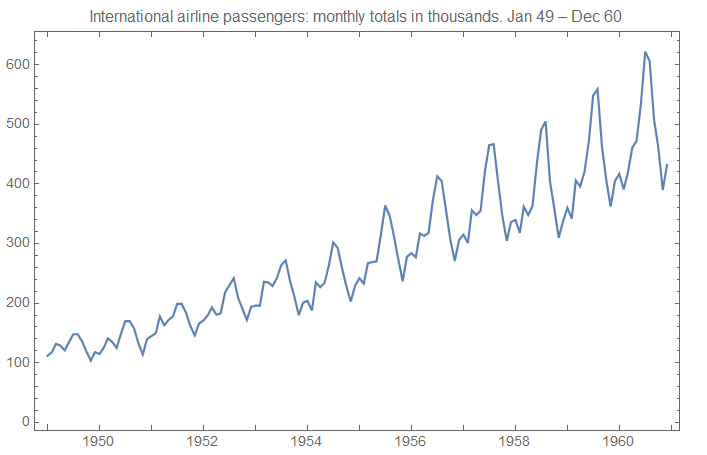
\includegraphics[scale=0.6]{pictures/1.png}
\end{center}

В качестве базовой группы, с которой ведется сравнение уровня занятости ручным трудом, выступают предприятия с низким уровнем автоматизации.

Регрессионная модель, исходя из средних уровней, составит:
$$\hat{y} = 56 - 21z_1 - 9.5z_2$$

Данная модель говорит, что на предприятиях с низким уровнем автоматизации средний процент рабочих, занятых ручным трудом, равен $56$. На предприятих с высоким уровнем распростаненность ручного труда ниже на $35-56 = -21$ процентных пункта, а на предприятиях со средним уровнем - ниже на $46,5 - 56 = -9,5$ процентных пункта по сравнению с предприятиями третьей группы.

Подставив различные комбинации фиктивных переменных в уравнение регрессии, получим средние значения по группам (теоретическое $y$).

Поскольку коэффициенты при фиктивных переменных в модели, не содержащей других факторов, характеризуют по существу величину эффектов $i$-го уровня фактора $z$, то регрессионная модель по своему содержанию тождественна дисперсионной модели.

\newpage
\subsection{Регрессия с фиктивной зависимой переменной, интерпретация параметров}

Может возникнуть необходимость построить модель, в которой фиктивной переменной выступает результативный признак. Подобного вида модели применяются при обработке данных опросов. Зависимая переменная принимает два значения: да - $1$ и нет - $0$.

Модель такой зависимой переменной выглядит следующим образом:
$$y = a + b_1 \cdot x_1 + \ldots + b_n \cdot x_n + \varepsilon$$

Модель является \textit{вероятностной линейной моделью}. В ней $y$ принимает значения $1$ и $0$, которым соответствуют вероятности $p$ и $1-p$. Поэтому при решении находят оценку условной вероятности события $y$ при фиксированных значениях $x$. Кратко: $y$ - \textit{вероятность наступления события} при фиксированных средних значениях $x$.

\textbf{Пример:} $Y$ - вероятность использования технологии, $X$ - возраст оборудования.
$$Y = 0.85 - 0.03X$$
то есть с ростом возраста оборудования на год вероятность использования прогрессивной технологии снижается на $0.03$.

Метод наименьших квадратов для данных моделей не используется.


\newpage
\subsection{Критерий Грегори Чоу. Его значение для построения модели регрессии}

Данный тест применяется для оценки существенности различий моделей регрессии по разным выборкам и при наличии структурной неоднородности совокупности для возможности построения общего уравнения регрессии.

Пусть дана выборка объема $n$, кототрая разбита на две подвыборки объемом $n_1$ и $n_2$. Для выборки и каждой подвыборки рассматривается регрессионная модель:
$$Y = a + bX, \qquad Y_1 = a_1 + b_1X, \qquad Y_2 = a_2 + b_2X$$ 

Выдвигается нулевая гипотеза:
$$H_0: b = b_1 = b_2$$
то есть для прогнозирования достаточно общей модели регрессии, разбиение на две модели не поспособствовало лучшему прогнозированию.

Альтернативной гипотезой $H_1: b \neq b_1 \neq b_2$ является структурная неоднородность даннных, после которой делается вывод - либо оставить две модели, либо строить общую регрессию с включением фиктивной переменной.

Для проверки гипотезы для каждой модели строится остаточная сумма квадратов $SS_0, SS_1,SS_2$.

Если $H_0$ верна, то $SS_0 = SS_1 + SS_2$, иначе справедлива альтернативная гипотеза $H_1$.

Существенноть различий $SS_0$ и $SS_1 + SS_2$ проверяют через следующую $F$-статистику.
$$F  = \frac{SS_0 - (SS_1 + SS_2)}{SS_1 + SS_2} \cdot \frac{n_1+n_2-2m-2}{m+1}$$
где $m$ - число факторов модели регрессии.

Если $F > F_{table} (m+1, n-2m-2)$, то $H_0$ отклоняется и качество частных моделей регрессии превосходит качество общей модели и существенны различия коэффициентов регрессии в подвыборках, если меньше, то $H_0$ принимается и разбивать на подвыборки общую регрессию не имеет смысла.
\newpage

\section{Системы эконометрических уравнений}

\subsection{Общее понятие о системах уравнений. Система одновременных уравнений}

Объектом статистического изучения в социальных науках являются сложные системы. Построение изолированных уравнений
регрессии недостаточно для описания таких систем и объяснения механизма их функционирования. Изменение одной переменной, как правило, не может происходить без изменения других. Поэтому важное место занимает проблема описания структуры связей между переменными системой так называемых одновременных уравнений.

Так, если изучается модель спроса как отношение цен и количества потребляемых товаров, то одновременно для прогнозирования спроса необходима модель предложения товаров, в которой рассматривается также взаимосвязь между количеством и ценой предлагаемых благ. Это позволяет достичь равновесия между спросом и предложением.

Системы уравнений может быть построена по-разному.

\textit{Система независимых переменных} - каждая независимая переменная $y$ рассматривается как функция одного и того же набора факторов $x$.
$$\left \{
\begin{matrix}
	y_1 = a_{11}x_1 + a_{12}x_2 + \ldots + a_{1m}x_m + \xi_1 \\[0.3cm]
	y_2 =a_{21}x_1 + a_{22}x_2 + \ldots + a_{2m}x_m + \xi_2  \\[0.3cm]
	\ldots \\
	y_n = a_{n1}x_1 + a_{n2}x_2 + \ldots + a_{nm}x_m + \xi_n 
\end{matrix}
\right.
$$
Набор факторов $x_i$ в каждом уравнении может варьироваться. Каждое уравнение может рассматриваться самостоятельно, для нахождения его параметров используется МНК. Каждое уравнение является уравнением регрессии.

Наибольшее распространение в эконометрических исследованиях получила \textbf{система одновременных (совместных, взаимозависимых) уравнений.} В ней одни и те же зависимые переменные в одних уравнениях входят в левую часть, а в других уравнениях – в правую часть:

$$\left \{
\begin{matrix}
	y_1 = b_{12}y_2 + b_{13}y_3 + \ldots + b_{1n}y_n +  a_{11}x_1 + a_{12}x_2 + \ldots + a_{1m}x_m + \xi_1 \\[0.3cm]
	y_2 =b_{21}y_1 + b_{23}y_3 + \ldots + b_{2n}y_n + a_{21}x_1 + a_{22}x_2 + \ldots + a_{2m}x_m + \xi_2  \\[0.3cm]
	\ldots \\
	y_n = b_{n1}y_1 + b_{n2}y_2 + \ldots + b_{n,n-1}y_{n-1} + a_{n1}x_1 + a_{n2}x_2 + \ldots + a_{nm}x_m + \xi_n 
\end{matrix}
\right.
$$

В эконометрике эта система уравнений называется также \textbf{структурной формой модели.} Для нахождения параметров каждого уравнения традиционный МНК неприменим, здесь используются специальные методы оценивания. В этом случае каждое из уравнений не может рассматриваться самостоятельно.


\newpage
\subsection{Структурная и приведенная форма модели: понятие и аналитический смысл}

Система одновременных уравнений (т.е структурная форма модели ) обычно содержит эндогенные и экзогенные переменные.
\textbf{Эндогенные переменные} – это зависимые переменные, число которых равно числу уравнений в системе. Они обозначаются через y.
\textbf{Экзогенные переменные} – это предопределенные переменные, влияющие на эндогенные переменные, но не зависящие от них. Они обозначаются через x.

Простейшая форма структурной модели имеет вид:
$$\left \{
\begin{matrix}
	y_1 = b_{12}y_2 + a_{11}x_1 + \xi_1\\
	y_2 = b_{21}y_2 + a_{22}x_2 + \xi_2
\end{matrix}
\right.
$$

$y_1,y_2$ - эндогенные переменные, их две,  $x_1,x_2$ - экзогенные переменные, влияют на $y_1, y_2$.

Классификация переменных на эндогенные и экзогенные зависит от теоретической концепции принятой модели. Экономические
переменные могут выступать в одних моделях как эндогенные, а в других - как экзогенные переменные. Внеэкономические переменные (например, климатические условия) входят в систему как экзогенные переменные. В качестве экзогенных переменных можно рассматривать значения эндогенных переменных за предшествующий период времени (лаговые переменные). Например, потребление текущего года $y_t$ может зависеть также и от уровня потребления в предыдущем году $y_{t-1}$.

Структурная форма модели позволяет увидеть влияние изменений любой экзогенной переменной на значения эндогенной переменной. Целесообразно в качестве экзогенных переменных выбирать такие переменные, которые могут быть объектом регулирования. Меняя их и управляя ими, можно заранее иметь целевые значения эндогенных переменных.

Коэффициенты $b_i$ при эндогенных и $a_j$ при экзогенных переменных называются \textbf{структурными коэффициентами модели}. Все переменные в модели могут быть выражены в отклонениях $x-\bar{x}$ и $y-\bar{y}$ от среднего уровня, поэтому свободный член в таких уравнениях отсутствует.

Использование МНК для оценивания структурных коэффициентов модели дает смещенные и несостоятельные оценки. Поэтому
обычно для определения структурных коэффициентов модели структурная форма преобразуется в приведенную.

\textbf{Приведенная форма модели} - система линейных функций эндогенных пременных от экзогенных.

$$\left \{
\begin{matrix}
	y_1 = \sigma_{11}x_1 + \sigma_{12}x_2 + \ldots + \sigma_{1m}x_m + \xi_1 \\[0.3cm]
	y_2 =\sigma_{21}x_1 + \sigma_{22}x_2 + \ldots + \sigma_{2m}x_m + \xi_2  \\[0.3cm]
	\ldots \\
	y_n = \sigma_{n1}x_1 + \sigma_{n2}x_2 + \ldots + \sigma_{nm}x_m + \xi_n 
\end{matrix}
\right.
$$
$\sigma_{ij}$ - коэффициенты приведенной формы модели.

По своему виду приведенная форма модели ничем не отличается от системы независимых уравнений, Применяя МНК, можно оценить $\sigma_{ij}$, а затем оценить значения эндогенных переменных через экзогенные.

Коэффициенты приведенной формы модели представляют собой \textit{нелинейные функции коэффициентов структурной модели}. Рассмотрим это на примере:

Простейшая форма структурной модели имеет вид:
$$\left \{
\begin{matrix}
	y_1 = b_{12}y_2 + a_{11}x_1\\
	y_2 = b_{21}y_2 + a_{22}x_2
\end{matrix}
\right.
$$

Приведенная форма структурной модели имеет вид:
$$\left \{
\begin{matrix}
	y_1 = \sigma_{11}x_1 + \sigma_{12}x_2\\
	y_2 = \sigma_{21}x_1 + \sigma_{22}x_2
\end{matrix}
\right.
$$

Из первого уравнения структурной модели
$$y_2 = \frac{y_1-a_{11}x_1}{b_{12}}$$

Тогда систему можно перезаписать:
$$ \frac{y_1-a_{11}x_1}{b_{12}} =  b_{21}y_2 + a_{22}x_2$$
$$y_1 - a_{11}x_1 = b_{12}b_{21}y_2 + a_{22}b_{12}x_2$$
$$y_1 \cdot (1-b_{12}b_{21]}) = a_{11}x_1 + a_{22}b_{12}x_2$$
$$y_1 = \frac{a_{11}}{1-b_{12}b_{21}}\cdot x_1 + \frac{ a_{22}b_{12}}{1-b_{12}b_{21}}\cdot x_2$$

Таким образом мы представли первое уравнение в виде уравнения приведенной формы модели:
$$y_1 = \sigma_{11}x_1 + \sigma_{12}x_2$$

Из уравнения следует, что коэффициенты приведенной формы модели представляют собой нелинейные соотношения коэффициентов структурной модели, т.е
$$\sigma_{11} =  \frac{a_{11}}{1-b_{12}b_{21]}}, \sigma_{12} = \frac{ a_{22}b_{12}}{1-b_{12}b_{21]}}$$

Аналогично поступим со вторым уравнением, получая:
$$y_2 = \frac{a_{11}b_{21}}{1-b_{12}b_{21}}\cdot x_1 + \frac{ a_{22}}{1-b_{12}b_{21}}\cdot x_2$$

С соответствующими коэффициентами $\sigma_{21} =  \frac{a_{11}b_{21}}{1-b_{12}b_{21}}, \sigma_{22} = \frac{ a_{22}}{1-b_{12}b_{21}}$

Приведенная форма позволяет выразить значения эндогенных переменных через экзогенные, однако аналитически уступает структурной форме модели, т.к. в ней отсутствуют оценки взаимосвязи между эндогенными переменными.


\newpage
\subsection{Проблема идентификации}

\subsubsection{Идентификация системы эконометрических уравнений, порядковое условие идентификации}
При переходе от приведенной формы модели к структурной исследователь сталкивается с проблемой идентификации.

\textbf{Идентификация} – это \textit{единственность соответствия} между приведенной и структурной формами модели.

Структурная модель в полном виде, состоящая в каждом уравнении из $n$ эндогенных и $m$ экзогенных переменных, содержит $n\cdot(n-1+m)$ параметров. Приведенная модель в полном виде содержит $nm$ параметров. В полном виде структурная модель содержит большее число параметров, чем приведенная форма модели. Поэтому $n\cdot(n-1+m)$ параметров не могут быть одноначно определены через $nm$ параметров приведенной формы модели.

Чтобы получить единственно возможное решение для структурной модели, необходимо предположить, что некоторые из структурных коэффициентов модели равны нулю. Тем самым уменьшится число структурных коэффициентов.

С позиции идентифицируемости структурные модели можно подразделить на три вида:

\begin{itemize}
	\item идентифицируемые
	\item неидентифицируемые
	\item сверхидентифицируемы
\end{itemize}

Модель \textbf{идентифицируема}, если все структурные ее коэффициенты определяются однозначно, единственным образом по коэффициентам приведенной формы модели, т.е. число параметров структурной модели \textbf{равно} числу параметров приведенной формы модели.

Модель неидентифицируема, если число приведенных коэффициентов \textbf{меньше числа структурных коэффициентов}, и в результате структурные коэффициенты не могут быть оценены через коэффициенты приведенной формы модели. Структурная модель в полном виде всегда неидентифицируема.

Модель сверхидентифицируема, если число приведенных коэффициентов \textbf{больше числа структурных коэффициентов.} В этом случае на основе приведенных коэффициентов можно получить два или более значений одного структурного коэффициента. Сверхидентифицируемая модель, в отличие от неидентифицируемой, практически решаема, но требует для этого специальных методов исчисления параметров.

Структурная модель всегда представляет собой систему совместных уравнений, каждое из которых требуется проверять на идентификацию. \textbf{Модель считается идентифицируемой, если каждое уравнение системы идентифицируемо.} Если хотя бы одно из уравнений системы неидентифицируемо, то и вся модель считается неидентифицируемой. 

Сверхидентифицируемая модель содержит \textit{хотя бы одно сверхидентифицируемое уравнение}.

Обозначим за $H$ - чиcло эндогенных переменных в $i$-м уравнении системы, $D$ - число экзогенных переменных, которые содержатся в системе, но не входят в уравнение. 

\textbf{Условие идентифицируемости уравнения}

\begin{itemize}
	\item $D+1 = H$ - уравнение идентифицируемо
	\item $D+1 < H$ - уравнение неидентифицируемо
	\item $D+1 > H$ - уравнение сверхидентифицируемо
\end{itemize}

Это счетное правило отражает необходимое, но не достаточное условие идентификации. Более точно условия идентификации определяются, если накладывать ограничения на коэффициенты матриц параметров структурной модели. 

\textit{Уравнение идентифицируемо}, если по отсутствующим в нем переменным (эндогенным и экзогенным) можно из коэффициентов при них в других уравнениях системы получить матрицу, определитель которой не равен нулю, а ранг матрицы не меньше, чем число эндогенных переменных в системе без одного.

$$Rank(M) \geq E-1$$

где $E$ - количество эндогенных переменных в системе.

Целесообразность проверки условия идентификации модели через определитель матрицы коэффициентов, отсутствующих в данном уравнении, но присутствующих в других уравнениях, объясняется тем, что возможна ситуаций, когда для каждого уравнение системы выполнено счетное правило, а определитель матрицы названных коэффициентов равен нулю. В этом случае соблюдается лишь необходимое, но недостаточное условие идентификации.

Обратимся к следующей структурной модели:
$$\left \{
\begin{matrix}
	\hat{y_1} = b_{12}y_2 + b_{13}y_3  +  a_{11}x_1 + a_{12}x_2\\
	\hat{y_2} = b_{21}y_1 + a_{22}x_2  +  a_{23}x_3 + a_{24}x_4\\
	\hat{y_3} = b_{31}y_2 + b_{32}y_2  +  a_{31}x_1 + a_{32}x_2

\end{matrix}
\right.
$$

Проверим каждое уравнение на необходимое и достаточное условие идентификации:

1. Первое уравнение: $H=3, D = 2, H = 2 + 1$, уравнение идентифицируемо

Для проверки на достаточное условие заполним следующую таблицу коэффициентв при отсутсвующих в первом уравнении переменных ($x_3,x_4$).

$$\left \{
\begin{matrix}
	n & x_3 & x_4 \\
	2 & a_{23} & a_{24} \\
	3 & 0 & 0 

\end{matrix}
\right \}
$$

Следовательно, определитель равен нулю и первое уравнение не идентифицируемо.

2. Второе уравнение: $H=2, D = 1, 2 = 1 + 1$, уравнение идентифицируемо. Достаточное выполняется.

$$\left \{
\begin{matrix}
	n & y_3 & x_1 \\
	1 & b_{13} & a_{11} \\
	3 & -1 & a_{31} 

\end{matrix}
\right \}
$$

Определитель не равен нулю, ранг матрицы равен двум, что не меньше числа эндогенных переменных без одной. $2=2$. Уравнение идентифицируемо.

3. Необходимое условие - идентифицируемо, достаточное - определитель не равен нулю.

\subsection{Методы оценки параметров структурной модели}

Коэффициенты структурной модели могут быть оценены разными способами в зависимости от вида системы одновременных
уравнений. Наибольшее распространение получили два метода оценивания коэффициентов структурной модели: \textit{косвенный МНК} и \textit{двухшаговый МНК}.

\subsubsection{Косвенный метод наименьших квадратов, условия и методика применения}

Косвенный МНК (КМНК) применим в случае \textit{точно идентифицируемой структурной модели.} Процедура следующая:

\begin{enumerate}
	\item Структурная модель преобразуется в приведенную форму
	\item Для каждого уравнения приведенной формы обычным МНК оцениваются коэффициенты $\sigma_{ij}$
	\item Коэффициенты приведенной модели трансормируются в параметры структурной модели.
\end{enumerate}

\subsubsection{Двухшаговый метод наименьших квадратов. Условия использования}

ДМНК используется для \textit{сверхидентифицируемых систем.} 

Основная идея ДМНК: на основе приведенной формы модели получить для сверхидентифицируемого уравнения теоретические значения эндогенных переменных, содержащихся в правой части уравнения. Далее, подставив их вместо фактических значений, можно применить обычный МНК к структурной форме сверхидентифицируемого уравнения. 

Здесь дважды используется МНК: на первом шаге при определении приведенной формы модели и нахождении на ее основе оценок теоретических значений эндогенной переменной $y_i = \sigma_{i1}x_1 + \sigma_{i2}x_2 + \ldots + \sigma_{im}x_m $ и на втором шаге применительно к структурному сверхидентифицируемому уравнению при определении
структурных коэффициентов модели по данным теоретических (расчетных) значений эндогенных переменных.

Сверхидентифицируемая структурная модель может быть двух типов:

\begin{itemize}
	\item все уравнения сверхидентифицируемые
	\item система содержит также точно идентифицируемые уравнения
\end{itemize}

В первом случае для оценки структурных коэффициентов каждого уравнения используется ДМНК. Во втором - структурные коэффициенты для точно идентифицируемых уравнений находятся из системы приведенных уравнений.

\newpage
\subsection{Применение систем эконометрических уравнений}

\subsubsection{Модели кейнсианского типа в эконометрике}

Наиболее широко системы одновременных уравнений используются при построении макроэкономических моделей экономики страны. В большинстве случае это мультипликаторные модели кейнсианского типа. Статическая модель Кейнс народного хозяйста в самом простом виде следующая:
$$\begin{cases}
	C = a + by + \varepsilon \\
	y = C + I
\end{cases}$$
где $C$ - личное потребление, $y$ - национальный доход в постоянных ценах, $I$ - инвестиции в постоянных ценах.

$b\leq 1$ - предельная склонность к потреблению, $a$ - прирост потребления за счет других факторов.

Эта модель точно идентифицируема и для получения $b$ применяется косвенный метод наименьших квадратов.

Структурный коэффициент $b$ используется для расчета мультипликаторов. По данной функции потребления можно определить два мультипликатора - инвестиционный мультипликатор потребления $M_c$ и нацинального дохода $M_y$:
$$M_c = \frac{b}{1-b}, \qquad M_y = \frac{1}{1-b}$$

В более поздних исследованиях статическая модель Кейнса включала не только функцию потребления, но и функцию сбережений:
$$\begin{cases}
	C = a + by + \varepsilon \\
	r = T + K \cdot (C + I) + \varepsilon_2 \\
	y = C + I - r \\
\end{cases}$$
где $r$ - сбережения.

Здесь три эндогенные переменные $C,r,y$ и одна экзогенная $I$. 

Система идентифицируема: в первом уравнении $H=2, D = 1, D + 1 = H$, во втором уравнении $H=1, D = 0, D + 1 = H$, в третьем уравнении $H=2, D=1, D + 1 = H$. $C+I$ рассматривается как предопределенная переменная.

\subsubsection{Модели Клейна, их назначение}

Наряду со статическими широкое распространение получили динамические модели экономики. Они содержат в правой части лаговые переменные, а также учитывают тенденцию. Например, модель Клейна экономики США 1950-1960 гг. в упрощенном варианте:
$$\begin{cases}
	C_t = b_1 \cdot S_t + b_2P_t + b_3 + \varepsilon_1 \\
	I_t = b_4P_t + b_5P_{t-1} + b_6 + \varepsilon_2 \\
	S_t = b_7R_t + b_8R_{t-1}+b_9t+b_{10} + \varepsilon_3\\
	R_t = S_t + P_t + T_t \\
	R_t = C_t + I_t + G_t
\end{cases}$$

где $T_t$ - чистые трансферты в пользу администрации

$I_t$ - капитальные вложения

$G_t$ - правительственные расходы

$S_t$ - заработная плата в период $t$

$P_t$ - прибыль

$P_{t-1}$ - прибыль в период $t-1$

$R_t$ - общий доход.

Модель содерижт $5$ эндогенных переменных - $C_t,I_t,S_t,R_t$ и $P_t$ - зависимая переменная, определяемая по тождеству, три экзогенные переменные $T_t,G_t,t$ и две лаговые предопределенные переменные $P_{t-1}$ и $R_{t-1}$. Данная модель сверхидентифицируема и решается ДМНК. Для прогнозных целей используется приведенная форма модели:
$$\begin{cases}
	C_t = d_1T + d_2 G +d_3T +d_4P_{t-1} +d_5R_{t-1} +U_1 \\
	I_t = d_6T + d_7 G +d_8T +d_9P_{t-1} +d_{10}R_{t-1} +U_2 \\
	S_t = d_{11}T + d_{12} G +d_{13}T +d_{14}P_{t-1} +d_{15}R_{t-1} +U_3 \\
	R_t = d_{16}T + d_{17} G +d_{18}T +d_{19}P_{t-1} +d_{20}R_{t-1} +U_4 \\
	P_t = d_{21}T + d_{22} G +d_{23}T +d_{24}P_{t-1} +d_{25}R_{t-1} +U_5 \\
\end{cases}$$

Здесь мультипликаторами являются коэффициенты при экзогенных переменных. Они отражают влияние экзогенной переменной
на эндогенную переменную.

\subsubsection{Модели спроса и предложения}

Система одновременных уравнений нашла применение в исследованиях спроса и предложения. Линейная модель спроса и предложения иметт вид:
$$\begin{cases}
	Q^d = a_0 + a_1P + \varepsilon_1 - \text{ объем спроса} \\
	Q^s = b_0 + b_1P + \varepsilon_2 - \text{ объем предложения} \\
	Q^d = Q^s 
\end{cases}$$

Здесь $3$ эндогенные переменные: $Q^d,Q^s, P$. $P$ - эндогенная по экономическому содержанию (цена зависит от спроса и предложения), а также в результате тождества:
$$a_0 + a_1P + \varepsilon_1 = b_0 + b_1P + \varepsilon_2$$
$$P = \frac{b_0-a_0}{a_1-b_1} + \frac{\varepsilon_2- \varepsilon_1}{a_1-b_1}$$

Модель не содержит экзогенной переменной. Однако, чтобы модель имела статистическое решение и можно было убедиться в ее справедливости, в модель вводятся экзогенные переменные.

Например, модель вида:
$$\begin{cases}
	Q^d = a_0 + a_1P + a_2R + \varepsilon_1 \\
	Q^s = b_0 + b_1P + b_2W + \varepsilon_2 \\
	Q^d = Q^s 
\end{cases}$$
где $R$ - доход на душу населения, а $W$ - климатические условия.

Переменные $R,W$ - экзогенные. Введя их в модель, получаем идентифицированную структурную модель, где можно применить косвенный метод наименьших квадратов (КМНК).

\newpage
\section{Временные ряды}

\subsection{Особенности эконометрического моделирования рядов}

\begin{definition}
	\textit{Временной ряд} – это совокупность значений какого – либо показателя за несколько последовательных моментов или периодов времени. Каждое значение (уровень) временного ряда формируется под воздействием большого числа факторов, которые можно условно разделить на три группы:
	\begin{itemize}
		\item факторы, формирующие тенденцию ряда;
		\item факторы, формирующие циклические колебания ряда;
		\item случайные факторы
	\end{itemize}

\end{definition}

1. Большинство временных рядов экономических показателей имеют \textit{тенденцию}. Тенденция характеризует долговременное воздействие факторов на динамику показателя. Тенденция может быть \textit{возрастающей} или \textit{убывающей}.

2. Изучаемый показатель может быть подвержен \textit{циклическим колебаниям.} Эти колебания могут носить сезонный характер, поскольку экономическая деятельность ряда отраслей зависит от времени года. Также могут отражать динамику коъюнктуры рынка, а также фазу бизнес-цикла, в которой находится экономика страны.

3. \textit{Случайная компонента} или \textit{остатки}

Чаще всего реальные данные содержат все три компоненты. Каждый их уровень формируется под воздействием тенденции, сезонных колебаний и случайной компоненты.

В большинстве случаев временной ряд можно представить как сумму или произведение трендовой $T$, циклической $S$ и случайной $E$ компонент. 

\begin{definition}
	В случае суммы имеет место \textit{аддитивная модель} временного радя:
	$$y = T + S + E$$
\end{definition}

\begin{definition}
	В случае произведения имеет место \textit{мультипликативная модель} временного ряда:
	$$y = T \cdot S \cdot E$$
\end{definition}

\textbf{Основная задача эконометрического исследования отдельного временного ряда} – выявление количественного выражения каждой из компонент и использование полученной информации для прогноза будущих значений ряда или построение модели взаимосвязи двух или более временных рядов.

\newpage
\subsection{Автокорреляция: понятие, аналитическое значение, использование}

Рассмотрим основные подходы к анализу отдельного временного ряда. 

Ряд может содержать, помимо случайной составляющей, либо тенденцию, либо только сезонную компоненту, либо все компоненты вместе. Для того, чтобы выявить наличие той или иной неслучайной компоненты, исследуется корреляционная зависимость между последовательными уровнями временного ряда или \textbf{автокорреляция уровней ряда}.

Основная идея - при наличии тенденции и циклических колебаний, значения каждого последующего уровня ряда зависят от предыдущих.

Количественно \textit{автокорреляцию} можно измерить с помощью линейного коэффициента корреляции между уровнями исходного временного ряда и уровнями ряда, сдвинутыми на несколько шагов во времени.

Коэффициент автокорреляции уровней ряда \textit{первого порядка} измеряет зависимость между соседними уровнями ряда $t$ и $t-1$, то есть при \textit{лаге} $1$.

Он вычисляется по формуле выборочного коэффициент корреляции:
$$r_{xy} = \frac{\sum(x_i-\bar{x})(y_i - \bar{y})}{\sqrt{\sum(x_i - \bar{x})^2}\sqrt{\sum(y_i - \bar{y})^2}}$$
где в качетсве $x$ берется ряд $y_2,\ldots,y_n$, а в качестве $y$ ряд $y_1,\ldots,y_{n-1}$.

$$r_1 = \frac{\sum\limits_{t=2}^n (y_t - \bar{y}_1)(y_{t-1}-\bar{y}_2)}{\sqrt{\sum\limits_{t=2}^n (y_t - \bar{y}_1)^2 }\sqrt{\sum\limits_{t=2}^n (y_{t-1} - \bar{y}_2)^2 }}$$
где в качестве средних величиен берутся значения:
$$\bar{y}_1 = \frac{\sum\limits_{t=2}^n y_t}{n-1}$$
$$\bar{y}_2 = \frac{\sum\limits_{t=2}^n y_{t-1}}{n-1}$$

Если значение коэффициента автокорреляции близко к единице, это указывает на очень тесную зависимость между соседними уровнями временного ряда и о наличии во временном ряде сильной линейной тенденции.

Аналогично определяются коэффициенты автокорреляции более высоких порядков.

\begin{definition}
	Число периодов, по которым рассчитывается коэффициент автокорреляции, называется \textit{лагом}.
\end{definition}

С увеличением лага число пар значений, по которым определяется коэффициент автокорреляции, уменьшается. Для обеспечения статистической достоверности максимальный лаг не должен превышать \textit{четверти общего объема выборки}.

\textbf{Свойства автокорреляции}

1. Коэффициент автокорреляции строится по аналогии с линейным коэффициентом корреляции, поэтому он характеризует тесноту \textit{только линейной связи} текущего и предыдущего уровня. Для временных рядов с нелинейной тенденции, коэффициент автокорреляции будет близок к $0$, хотя тенденция все же в ряде есть.

2. По знаку коэффициента автокорреляции \textit{нельзя} делать выпод о возрастающей или убывающей тенденции в уровнях ряда.

\begin{definition}
	Последовательность коэффициентов автокорреляции уровней различных порядков, начиная с первого, называется \textit{автокорреляционной функцией временного ряда}.
\end{definition}

\begin{definition}
	График зависимости автокорреляционной функции от величины лага называется \textit{коррелограммой}.
\end{definition}

Анализ автокорреляционной функции позволяет определить лаг, при котором автокорреляция наиболее высокая, лаг, при котором связь между текущим и предыдущим уровнями ряда наиболее тесная.

\textbf{Анализ коррелограммы}

1. Если наиболее высоким является коэффициент автокорреляции первого порядка, то исследуемый ряд содержит \textit{только тенденцию}.

2. Есди наиболее высоким оказался коэффициент автокорреляции \textit{второго порядка}, то ряд содержит циклические колебания с циклом, равным двум периодам времени, то есть имеет \textit{пилообразную структуру}.

3. Если наиболее высоким оказался коэффициент автокорреляции порядка $\tau$, то ряд содержит циклические колебания с периодичностью в $\tau$ моментов времени.

4. Если ни один из коэффициентов $\tau$ не является значимым, то либо ряд не содержит тенденции и циклических колебаний и имеет только случайную составляющую, либо содержит сильную нелинейную связь, для исследования которой нужно провести дополнительный анализ.

\newpage
\subsection{Моделирование тенденции временного ряда}

\subsubsection{Основные типы трендов, используемых при аналитическом выравнивании, методика выбора формы уравнения}

Способ моделирования тенденции - построение аналитической функции, характеризующей зависимость уровней ряда от времени или тренда.

\begin{definition}
	Данный способ моделирования тендцении называется \textit{аналитическим выравниванием временного ряда}.
\end{definition}

Зависимость от времени может принимать разные формы, поэтому для ее формализации можно использовать различные виды функций. Для построения тренда чаще всего применяются следующие функции:

\begin{itemize}
	\item линейный тренд $\hat{y}_t = a + b\cdot t$
	\item гипербола $\hat{y}_t = a + \frac{b}{t}$
	\item экспоненциальный тренд $\hat{y}_t = e^{a+b\cdot t}$ или $\hat{y}_t = a \cdot b^t$
	\item степенной тренд: $\hat{y}_t = a \cdot t^b$
	\item параболический тренд второго и более высоких порядков:
	$$\hat{y}_t = a + b_1 \cdot t + b_2 \cdot t^2 + \ldots + b_k \cdot t^k$$
\end{itemize}

Параметры каждого из трендов можно определит обычным МНК, используя в качестве независимой переменной время, а в качестве зависимой - $y_t$ - уровни временного ряда (или уровни за вычетом цилической составляющей, если обнаружена). Для нелинейных трендов проводят стандартную процедуру их линеаризации.

\subsubsection{Выбор вида уравнения тренда. Оценка качества уравнения тренда}

\textbf{Выбор вида уравнения тренда}

1. Визуальный график зависимости уровней ряда от времени

2. Автокорреляция уровней ряда. Если временной ряд имеет линейную тенденцию, то его соседние уровни тесно коррелируют. В этом случае коэффициент автокорреляции первого порядка уровней исходного ряда должен быть высоким.

3. Если нелинейная тендценция, например, в форме экспоненты, то коэффициент автокорреляции первого порядка по логарифмам уровней исходного ряда будет выше, чем соответствюущий коэффициент, расчитанный по уровням ряда. Чем сильнее нелинейная тенденция - тем в больше степени будут различаться значения указанных коэффициентов.

\textbf{Оценка качества уравнения тренда}

Выбор лучшего уравнения тренда - расчет по каждому скорректированного коэффициента детерминации $\hat{R}^2$ и выбора уравнения тренда с максимальным значением этого коэффициента.

Экономическая интерпретация при линейном тренде - $a$ - начальный уровень временного ряда, $b$ - средний за период абсолютный прирост уровней ряда.

При экспоненциальном тренде - $a$ - начальный уровень временного ряда, $e^b$ - средний за единицу времени коэффициент роста уровней ряда.

\subsubsection{Точечный и интервальный прогноз на основе уравнения тренда}

Точечный и интервальный прогноз вычисляется абсолютно так же, как и при модели парной регрессии, а именно вычисляется стандартная ошибка, вычисляется предельная ошибка, домножается на квантили распределения Стюдента с $n-2$ степенями свободы и $\pm$ к точечному прознозному значению  - так будет построен и точечный прогноз, и интервальный прогноз.

Во всех подробностях построение интервального прогноза было рассказано в параграфе $1.10$, поэтому мы не будем повторяться, а просто напомнили основные этапы построения.

\newpage
\subsection{Моделирование сезонных колебаний. Аддитивные и мультипликативные модели в измерении сезонных колебаний}

При анализе временных рядов, содержащих сезонные или циклические колебания, наиболее простым подходом является расчет значений сезонной компоненты методом скользящего среднего и построение аддитивной или мультипликативной модели временного ряда:
$$Y  = T + S + E, \qquad  Y = T \cdot S \cdot E$$

Выбор одной из двух моделей проводится на основе анализа структуры сезонных колебаний:

Если амплитуда колебаний приблизительно постоянна, то строят аддитивную модель, в которой значения сезонной компоненты предполагаются постоянными для различных циклов.

Если амплитуда сезонных колебаний возрастает или уменьшается, то строят мультипликативную модель, которая ставит уровни ряда в зависимость от значений сезонной компоненты.

Построение аддитивной и мультипликативной модели сводится к расчету значений $T, S, E$ для каждого уровня ряда.

Процесс построения включает в себя следующее:

\begin{enumerate}
	\item Выравнивание исходного ряда методом скользящей средней.
	\item Расчет значений сезонной компоненты $S$
	\item Устранение сезонной компоненты из исходных уровней ряда и получение выровненных данных $(T+E)$ в аддитивной или $(T \cdot E)$ в мультипликативной модели.
	\item Аналитическое выравнивание уровней $(T+E)$ или $(T \cdot E)$ и расчет значений $T$ с использованием полученного уравнения тренда.
	\item Расчет полученных по модели значений $(T+S)$ или $(T \cdot S)$
	\item Расчет абсолютных и относительных ошибок
\end{enumerate}

Если полученные значения ошибок не содержат автокорреляции, ими можно заменить исходные уровни ряда и в дальнейшем использовать временной ряд ошибок $E$ для анализа взаимосвязи исходного ряда и других временных рядов.

\textbf{Аддитивные модели в измерении сезонных колебаний}

Сначала выравниваем исходный ряд методом скользящей средней, потом высчитываем сезонную компоненту и вычитаем ее из ряда, получаем $T+E = Y-S$ в аддитивной модели. Затем находим уравнение тренда, делаем аналитическое выравнивание уровней $Y-S = T+E$ с использованием уравнения тренда. После этого получим случайные компоненты путем вычитания $E = Y - (S+T)$ - это и есть расчет ошибки.

\textbf{Мультипликативные модели в измерении сезонных колебаний}

Сначала выравниваем исходный ряд методом скользящей средней, потом высчитываем сезонную компоненту и убираем ее из ряда, получаем $TE = \frac{Y}{S}$ в мультипликативной модели. Затем находим уравнение тренда, делаем аналитическое выравнивание уровней $\frac{Y}{S} = TE$ с использованием уравнения тренда. 

Расчет ошибки в мультипликативной модели проводится по формуле:
$$E = \frac{Y}{ST}$$

Абсолютные ошибки определяются как $E = y_t - T\cdot S$
\subsubsection{Фиктивные переменные в учёте сезонности при построении эконометрических моделей}

Рассмотрим еще один метод моделирования временного радя, содержащего сезонные колебания - построение модели регрессии с включением фактора времени и фиктивных переменных.

Количество фиктивных переменных в такой модели должно быть на единицу меньше числа периодов времени внутри одного цикла колебаний. Например, при моделированни поквартальных данных модель включает четыре независимые переменные - фактор времени и три фиктивные переменные.

Каждая фиктивная переменная отражает сезонную (циклическую) компоненту временного ряда для какого-либо одного периода. Она равна $1$ для данного периода и $0$ для всех остальных периодов.

Пусть имеется временной ряд, содержащий циклические колебания периодичностью $4$. Модель регрессии с фиктивными переменными для этого ряда будет иметь вид:
$$y_t = a + bt + c_1x_1+ c_2x_2 + c_3x_3 + \varepsilon_t$$
где $x_1$ - $1$ для первого квартала, $0$ для других кварталов и так далее.

Уравнение тренда для каждого квартала будет иметь следующий вид:
$$y_t = a + b\cdot t + c_1 + \varepsilon_t, (1)$$
$$y_t = a + b\cdot t + c_2 + \varepsilon_t, (2)$$
$$y_t = a + b\cdot t + c_3 + \varepsilon_t, (3)$$
$$y_t = a + b\cdot t + \varepsilon_t, (4)$$

Таким образом, фиктивные переменные позволяют дифференцировать величину свободного члена уравнения регрессии для каждого квартала. Она составит:
$$a+c_1,a+c_2,a+c_3,a$$
для кварталов с номерами $[1:4]$.

Параметр $b$ в этой модели характериует среднее абсолютное изменение уровней ряда под воздействием тенденции. В сущности модель есть аналог аддитивной модели временного ряда - это сумма трендовой, сезонной и случайной компонент.

Основной недостаток модели с фиктивными переменными для описания сезонных и циклических колебаний - наличие большого количества переменных. В такой ситуации количество степеней свободы невелико, что снижает вероятность получения статистически значимых оценок параметров уравнения регрессии.

\newpage
\subsection{Автокореляция остатков и ее роль при построении моделей регрессии}

Рассмотрим уравнение регрессии вида:
$$y_t = a + \sum\limits_{j=1}^k b_j \cdot x_{ji} + \xi_j$$
где $k$ - число независимых переменных.

Для каждого момента времени значение коммпоненты остатка определяется как:
$$\xi_t = y_t - \hat{y}_t = y_t - ( a + \sum\limits_{j=1}^k b_j \cdot x_{ji})$$

Рассматривая последовательност остатков как временной ряд, можно построить график из зависимости от времени. В соответствии с предпосылками МНК остатки должны быть случайными, однако при моделировании временных рядов нередко встречаются ситуации, когда остатки содержат тенденцию или колебания. Это свидетельствует о том, что каждое следующее значение остатков зависит от предыдущих.

\begin{definition}
	В этом случае говорят о наличии \textit{автокорреляции в остатках}
\end{definition}

Автокорреляция остатков может быть вызвана несколькими причинами, имеющих различную природу: ошибки измерения, в формулировке модели, когда модель не включает фактор, оказывающий существенное влияние на результат, влияние которого отражается в остатках (очень часто этот фактор - $t$ либо лаговые).

Известны два метода определения автокорреляции в остатках. 

Первый метод - построение графика зависимости остатков от времени и визуальное определение наличия или отсутствия автокорреляции. Второй метод - использование критерия \textit{Дарбина-Уотсона}.

\subsubsection{Критерий Дарбина-Уотсона и его применение}

Расчитывается величина:
$$d = \frac{\sum\limits_{i=2}^n (\xi_t - \xi_{t-1})^2}{\sum\limits_{t=1}^n \xi_t^2}$$

Таким образом, $d$ - отношение суммы квадратов разностей последовательных значений остатков к остаточной сумме квадратов модели регрессии. 

Коэффициент автокорреляции остатков первого порядка определяется как:
$$r_1^{\xi} = \frac{\sum\limits_{t=2}^n (\xi_t - \bar{\xi}_1)(\xi_{t-1}-\bar{\xi}_2)}{\sqrt{\sum\limits_{t=2}^n (\xi_t - \bar{\xi}_1)^2 }\sqrt{\sum\limits_{t=2}^n (\xi_{t-1} - \bar{\xi}_2)^2 }}$$
где в качестве средних величин берутся значения:
$$\bar{\xi}_1 = \frac{\sum\limits_{t=2}^n \xi_t}{n-1}$$
$$\bar{\xi}_2 = \frac{\sum\limits_{t=2}^n \xi_{t-1}}{n-1}$$

Параметры определялись по МНК, в соответствии сумма и среднее значение остатков равны $0$. Следовательно:
$$\bar{\xi}_1 = \bar{\xi}_2 = 0$$

Из этих выводов можно вывести следующее соотношение между критериями Дарбина-Уотсона и коэффициентом автокорреляции остатков первого периода:
$$d \approx 2 \cdot (1-r_1^{\xi})$$

Таким образом, если в остатках существует полная положительная автокорреляция, то $r_1^{\xi} = 1$ и $d=0$, если полная отрицательная автокорреляция,  то $r_1^{\xi} = -1$ и $d=4$. Если автокорреляци отсутствует,  то $r_1^{\xi} = 0$ и $d=2$. Следовательно:
$$0 \leq d \leq 4$$ 

\textbf{Алгоритм построения автокорреляции остатков на основе критерия Дарбина-Уотсона}

Выдвигается нулевая гипотеза $H_0$ об отсутствии автокорреляции в остатках. Альтернативные гипотезы $H_1$ и $H_1^*$ - наличие положительной ии отрицательной автокорреляции в остатках.

Далее определяются критические значения критерия Дарбина-Уотсона $d_L$ и $d_U$ для заданного числа наблюдений $n$, числа независимых переменных модели $k$ и уровня значимости $\alpha$.

При этом числовой промежуток $[0;4]$ разбивают на $5$ промежутков. Принятие или отклонение каждой из гипотез с вероятностью $1-\alpha$ представлено ниже:

\begin{center}
	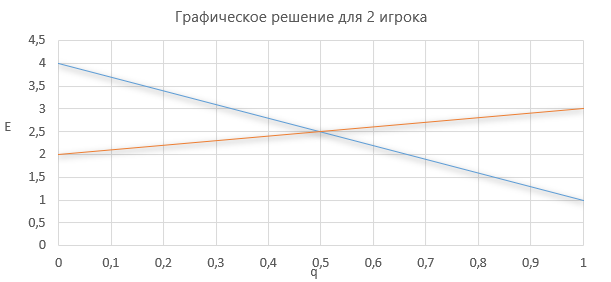
\includegraphics[scale=0.6]{pictures/2.png}
\end{center}

Если фактическое значение критерия Дарбина-Уотсона попадает в зону неопределености, то на практике предполагают существование автокорреляции остатков и отклоняют гипотезу $H_0$.

Критерий Дарбина-Уотсона неприним к моделям, включающим в качестве независимых переменных лаговые значения результативного признака, то есть к моделям авторегрессии.

Для тестирования на автокорреляцию остатков моделей авторегрессии используется критерий $h$ Дарбина.

\newpage
\section{Динамические модели}

\subsection{Особенности изучения взаимосвязей динамических рядов. Модели с лаговыми переменными. Их общая характеристика}

Теперь рассмотрим модели временных рядов, где в качестве исходных статистических данных мы располагаем наблюдениями \textit{двух временных рядов} $x_1,\ldots,x_n$ и $y_1,\ldots,y_n$. Целью регрессионного анализа в данном случае является построение линейной регрессионной модели, позволяющей с наименьшими ошибками прогнозировать значения $y_t$ по значениям $x_t$ для $t >n$.

Подобные модели естественны в ситуациях, когда две переменные x и y связаны так, что воздействия единовременного изменения одной из них $(x)$ на другую $(y)$ сказывается в течение достаточно продолжительного времени, т.е. наблюдается распределенный во времени эффект воздействия. В частности, такие связи возникают между регистрируемыми во времени входными и выходными характеристиками процессов накопления и распределения ресурсов (например, процессов преобразования доходов населения в его расходы) или процессов трансформации затрат в результаты (например, процессов
воспроизводства основных доходов).

Эконометрическая модель является \textit{динамической}, если в данный момент $t$ она учитывает значения входящих в неё переменных, относящихся как к текущему, так и к предыдущим моментам времени, т.е. модель учитывает, отражает динамику исследуемых переменных в каждый момент времени.

При исследовании экономических процессов нередко приходится моделировать ситуацию, когда значение результативного признака в текущий момент времени $t$ формируется под воздействием ряда факторов, действовавших в прошлые моменты времени $t-1,t-2,\ldots,t-l$.

\begin{definition}
	Переменные, влияние которых характеризуется определенным запаздываением, называются \textit{лаговыми переменными}.
\end{definition}
\begin{definition}
	Величину $l$, характеризующую запаздыванием в воздействии фактора на результат, в экнометрике называют \textit{лагом}. Временные ряды самих факторыных переменных, сдвинутые на один или более моментов времени - лаговыми переменными.
\end{definition}

Динамические модели классифицируют по-разному. Один из вариантов классификации следующий:

1. \textit{Регрессионные модели с распределенными лагами} содержат в качестве лаговых переменных лишь независимые (объясяющие) переменные, например:
$$y = a + b_0x_t + b_1x_{t-1} + b_2x_{t-2} + \xi_t$$

2. \textit{Авторегрессионные модели} - уравнения включают в качестве объясняющих переменных лаговые значения зависимых переменных,  то есть на величину зависимой переменной текущего периода могут оказывать влияние ее значения в прошлые моменты или периоды времени, например:
$$y = a + bx_t + c_1y_{t-1} + c_2y_{t-2} + \varepsilon_t$$

3. Модель с лаговой зависимой и независимой переменной - \textit{авторегрессионная модель с распределенными лагами}

Построение динамических моделей имеет свою специфику. Во-первых, оценка параметров моделей авторегресси, в большинстве случаев и моделей с распределенным лагом, не может быть проведено с помощью МНК из-за нарушения предпосылок и требует специаьных статистических методов. Во-вторых, нужно отбирать оптимальную величину лага и определения его структуры. В третьих, между моделями авторегрессии и распределенного лага существует связь и иногда нужно совершить переход от одной модели к другой.

\newpage
\subsection{Регрессионные модели с распределёнными лагами. Интерпретация параметров}

Динамические модели классифицируют по-разному. Один из вариантов классификации следующий.

\textit{Регрессионные модели с распределенными лагами} содержат в качестве лаговых переменных лишь независимые (объясяющие) переменные, например:
$$y = a + b_0x_t + b_1x_{t-1} + b_2x_{t-2} + \xi_t$$
является примером модели с распределенным лагом.

Рассмотрим модельс распределенным лагом в ее бщем виде в предположении, что максимальная величина лага конечна:
$$y_t = a + b_0x_t + b_1x_{t-1} + \ldots + b_p \cdot x_{t-p} + \varepsilon_t$$

Данная модель говорит о том, что если в некоторый момент времени $t$ происходит изменение независимой переменной $x$, то это изменение будет влиять на значения переменной $y$ в течение $l$ следующих моментов времени.

Коэффициент $b_0$ называется \textit{краткосрочным мультипликатором}, так как он характеризует изменение среднего значения $y$ при единичном изменении $x$ в тот же самый момент времени.

Сумма $\sum\limits_{j=0}^p b_j$ называется \textbf{долгосрочным мультипликатором}, так как он характеризует изменение $y$ под воздействием единичного изменения $x$ в каждом из моментов времени (абсолютное изменение в долгосрочном периоде $t+l$ результата $y$ под влиянием изменения на $1$ единицу фактора $x$).

Любая сумма $\sum\limits_{j=0}^k b_j, k <p$ называется \textbf{промежуточным мультипликатором}

\begin{definition}
	\textit{Относительные коэффициенты модели} с распределенным лагом определяются выражениями:
	$$\beta_j = \frac{b_j}{\sum\limits_{j=0}^p b_j}$$
\end{definition}

Если все коэффициенты $b_j$ имеют одинаковые знаки, то для любого $j$:
$$0 < \beta_j < 1, \qquad \sum\limits_{j=0}^l \beta_j = 1$$

В этом случае относительные коэффициенты $\beta_j$ являются весами для соответствующих коэффициентов $b_j$. Каждый из них измеряет долю общего изменения $y$ в момент времени $t+j$.

\begin{definition}
	\textit{Средний лаг} расчитывается по формуле арифметической взвешенной:
	$$\bar{l} = \sum\limits_{j=0}^l j \cdot \beta_j$$

	Он означает период, в течение которого происходит изменение результата от изменения $x$ в момент $t$. Небольшая величина означает быструю реакцию $y$ на изменение $x$, высокое - воздейсиве фактора $y$ будет сказываться в течение длительного времени.
\end{definition} 

\begin{definition}
	\textit{Медианный лаг} - это величина лага, для которого:
	$$\sum\limits_{j=0}^{l_{Me}} \beta_j \approx 0.5$$

	Это время, в течение которого с момента $t$ будет реализована половина общего воздействия фактора на результат.
\end{definition}

Применение МНК к таким моделям затруднительно по следующим причинам:

\begin{enumerate}
	\item Текущие и лаговые значения $x$ тесно связаны между собой, что приводит к высокой мультиколлинеарности факторов
\end{enumerate}
\begin{enumerate}
	\item При большой величине лага велико число параметров, что приводит к уменьшению числа степеней свободы
\end{enumerate}
\begin{enumerate}
	\item Часто возникает проблема автокорреляции остатков, что приводит к значительной неопределенности относительно оценок параметров модели, снижению точности и получению неэффективных оценок.
\end{enumerate}

Для получения более обоснованных оценок нужна информация о структуре лага. Эта структура может быть различной.

Если с ростом величина лага коэффициенты при лаговых переменных убывают, то имеет место линейная (или треугольная) структура лага, а также геометрическая структура. 

Рассмотрим некоторые подходы к расчету лагов.

\textbf{Лаги Алмон}

Предполагается, что воздействие коэффициентов при лаговых переменных с течением времени уменьшается и значения коэффициентов $b_j$ описываются полиномом $k$-й степени:
$$b_j = c_0 + c_1j + c_2j^2 + \ldots + c_kj^k$$

При этом априори выдвигается предположение о степени полинома. Как правило используется многочлен невысокой степени. Тогда:
$$y_t = a + c_0z_0 + c_1z_1 + c_2z_2 + \ldots + c_kz_k + \varepsilon_t$$

Параметры $c_j$ определяются по МНК.

Итого, процедура применения метода Алмон для расчета параметров модели с распределенным лагом выглядит следующим образом:

\begin{enumerate}
	\item Определяется максимальная величина лага $l$
	\item Определяется степень полинома $k$, описывающего структуру лага
	\item По соотношениям рассчитываются значения переменной $z_1,\ldots,z_k$
	\item Определяются параметры уравнения линейной регрессии по МНК
	\item С помощью соотношения расчитываются исходные параметры исходной модели с распределенным лагом
\end{enumerate}

Достоинства данного метода

\begin{itemize}
	\item Универсальность, применимость для моделирования процессов с разнообразными структурами лагов.
	\item При малом $k$ можно построить модели с распределенным лагом любой длины.
\end{itemize}

Ограничения методов

\begin{itemize}
	\item  Величина полинома должна быть известна заранее, при этом приходится задавать максимально возможную величину лага.
	\item Величина лага должна быть известна заранее
	\item Возможна мультиколлинеарность факторов $z_j$.
\end{itemize}

\textbf{Метод Койка}

Этот метод применяется в модели с бесконечным лагом:
$$y_t = a+b_0x_t + b_1x_{t-1} + \ldots + \xi_t$$

Здесь обычный МНК применить нельзя. Для идентификации модели предполагается, что параметры с увеличиением лага убывают в геометрической прогрессии, то есть с постоянным темпом $\lambda \in (0,1)$

Можно перейти к модели авторегрессии:
$$y_t = a(-\lambda) + b_0 x_t + \lambda y_{t-1} + u_t$$

Определив ее параметры находим $\lambda,a,b_0$ исходной модели, а затем и параметры $b_j = \lambda^j b_0, j = 1,2,3$. Данная модель позволяет определить долгосрочный мультипликатор $\sum\limits_{j=0}^{\infty} b_j = b_0 \frac{1}{1-\lambda}$ и средний лаг $\bar{l} = \frac{\lambda}{1-\lambda}$


\newpage
\subsection{Модели авторегрессии. Проблемы построения и интерпретация параметров}

\textit{Авторегрессионные модели} - уравнения включают в качестве объясняющих переменных лаговые значения зависимых переменных,  то есть на величину зависимой переменной текущего периода могут оказывать влияние ее значения в прошлые моменты или периоды времени, например:
$$y = a + b_0x_t + c_1y_{t-1} + c_2y_{t-2} + \varepsilon_t$$

$b_0$ в этой модели характеризует краткосрочное изменение $y_t$ под воздействием изменения $x_t$ на 1 единицу.

К моменту времени $t+1$ результат $y_t$ изменился под воздействием изменения изучаемого фактора в момент времени $t$ на $b_0$ единиц, а $y_{t+1}$ - под воздействием своего изменения в непосредственно предшествующий момент времени на $c_1$ единиц. В момент $t+1$ изменение результат составит $b_0c_1$ и.т.д

Следовательно, долгосрочный мультипликатор в модели авторегрессии можно рассчитать как сумму краткосрочного и промежуточного мультипликатора:
$$b = b_0 + b_0c_1 + b_0c_1^2 + b_0c_1^3 = \frac{b_0}{1-c_1}, \qquad |c_1| <1$$

\newpage
\subsection{Инструментальные переменные}

Метод инструментальных переменных предполагает, что раз в правой части модели авторегрессии поставлена лаговая объясняемая переменная, то нарушаются предпосылки МНК, ведь $y$ должен быть независим, а это не является правдой.

Суть метода состоит в том, что вместо лаговой зависимой переменной $y_{t-1}$, для которой нарушается предпосылка МНК, используется другая переменная $z_t$, называемая \textit{инструментальной}. При этом инструментальная переменная должна обладать двумя свойствами:

\begin{itemize}
	\item Она должна быть тесно коррелирована с лаговой зависимой еременной $y_{t-1}$
	\item Она не должна коррелировать с остатками $\xi_t$. 
\end{itemize} 

Иными словами от модели авторегрессии:
$$y_t = a + b_0x_t + c_1y_{t-1} + \xi_t$$
необходимо перейти к модели вида:
$$y_t = a + b_0x_t + cz_t + \xi_t$$

Результаты ререссии по модели зависят от того, насколько удачно подобана инструментальная переменная $z_t$. В качестве инструментальной переменной можно взять, например, \textit{оценки $y_{t-1}$}, то есть теоретические значения $y_{t-1}$, полученные по регрессии $y_{t-1}$ от $x_{t-1}$. 

Это связано с тем, что в исходной модли $Y_t$ связан с $x_t$, следовательно, можно предположить, что зависимость между $y_{t-1}$ и $x_{t-1}$ тоже существует:
$$\hat{y}_{t-1} = A + B x_{t-1}$$ 
и теперь к этой модели можно применить МНК. Метод похож на двухшаговый МНК.

\newpage

\subsection{Модели с периодическими колебаниями. Ряд Фурье по стационарному ряду}

Уровни ряда варьируют вокруг среднего значения $\bar{y}$, а их колебания повторяются.

\begin{definition}
	Интервал времени, необходимый, чтобы динамический рял начал повторяться, называется \textit{периодом} и обозначен на графике за $P$.
\end{definition}

Его величина (расстояние между пиками и впадинами) составляет $12-2=10$ месяцев. Если ряд имеет период $P$, то как правило, имеет также период $2P, 3P$ и.т.д

В общем случае для стационарного временного ряда справедливо равенство:
$$y_t = y_t + cp, c = 1,2$$

\begin{definition}
	Величина, обратная периоду, называется \textit{частотой динамического ряда}:
	$$f = \frac{1}{P}$$

	Частота указывает на число повторений цикла в единицу времени: $f = \frac{1}{10}$ в месяц. 
\end{definition}

\begin{definition}
	Отклонение от среднего уровня до пика называется \textit{амплитудой временного графика}, на графике - $A$.
\end{definition}

\begin{definition}
	Расстояние между началом отсчета времени $t=0$ и ближайшим пиковым значением называется \textit{фазой} (Ф).
\end{definition}

Стационарный периодический временной ряд можно задать четырьмя параметрами: периодом $P$ или частотой $f$, амплитудой $A$, фазой $\text{Ф}$ и средним значением $\bar{y}$, что может быть представлено:
$$y_t = \bar{y} + A \cdot \cos W(t-\text{Ф})$$
где $W$ - угловая частота, измеряемая в радианах в единицу времени и равна $W = 2\pi f,  0 \leq W \leq 2\pi$.

\begin{definition}
	Рассмотренное выражение называется \textit{гармоническим представлением ряда} и часто записывается через синусы и косинусы без упоминания о фазе:
	$$y_t = \bar{y} + a \cos Wt + b \sin Wt$$
	где $a = A \cos \Phi, b = A \sin \Phi$.
\end{definition}

Теоретически стационарный временной ряд с периодическими колебаниями может быть представлен как сумма среднего значения и ряда синусоид и косинусоид, что и называется \textit{рядом Фурье}:
$$y_t = \bar{y} + \sum\limits_{i=1}^{\infty}a_i \cos W_it + \sum\limits_{i=1}^{\infty}b_i \cos W_it$$

Анализируемые ряда динамики обычно имеют конечную длину $N$. Поэтому ряд Фурье преобретает вид:
$$y_t = \bar{y} + \sum\limits_{i=1}^{n}a_i \cos W_it + \sum\limits_{i=1}^{n}b_i \cos W_it$$
где $n = \frac{N}{2}$.

Заменив $\bar{y}$ параметром $a_0$, ряд Фурье принимает вид:
$$y_t = a_0 +  \sum\limits_{i=1}^{n}a_i \cos W_it + \sum\limits_{i=1}^{n}b_i \cos W_it$$

Оценка параметров данного уравнения обычно дается МНК. Покажем его применение для случая одной гармоники.
$$y_t = a_0 + a_1 \cos t + b_1 \sin t$$
где $t$ принимает значения от $0$ с последующим увеличением на $\frac{2\pi}{N}$.

Параметры гармонии определяются как:
$$a_1 = \frac{2\sum\limits y_t \cos t}{N}, \qquad b_1 = \frac{2\sum\limits y_t \sin t}{N}$$

Ряд Фурье с двумя гармониками:
$$y_t =  a_0 + a_1 \cos t + b_1 \sin t + a_2 \cos 2t + b_2 \sin 2t$$

\textbf{Ряд Фурье по рядам с тенденцией}

В этом случае при наличии периодических колебаний ряд Фурье может быть использован, если привести рял к стационарному виду. Для этой цели можно найти линейный тренд $\hat{y}_t = a + bt$ и применить ряд Фурье к остаточным величинам:
$e_t = y_t  -\hat{y}_t$

\newpage
\subsection{Модели регрессии по рядам динамики, особенности построения}

\subsubsection{Разложение уровня динамического ряда на компоненты. Мультипликативные и аддитивные модели}

\textbf{Аддитивная модель сезонности}

$y_t = \bar{y} + S + \varepsilon$ при отсутствии тендценции, $y_t = \hat{y}_t + S + \varepsilon$ - при наличии, где $y_t$ - уровень динамического ряда, а $\hat{y}_t$ - теоретический уровень ряда согласно тенденции, $S$ - сезонная составляющая, измеренная в тех же единицах, что и уровень ряда.

\textbf{Мультипликативная модель сезонности}

В пультипликативной модели уровень динамичнского ряда рассматривается как произведение его компонент:
$$y_t = \hat{y_t} \cdot K_s \cdot E_t$$
где $y_t$ - фактические уровни динамического ряда, $\hat{y}_t$ - теоретические значения уровней динамического ряда согласно тенденции, $K_s$ - коэффициент сезонности, $E_t$ - коэффициент случайной компоненты.

В данной модели $\hat{y}_t \cdot K_s$ представляет собой тренд с учетом сезонной волны $y_s$, то есть уровень ряда, обусловленный влиянием как тенденции, так и сезонности: $y_s = \hat{y}_t \cdot K_s$. Используя величину $y_s$, мультипликативную модель можно представить как:
$$y_t = \hat{y}_t \cdot \frac{y_s}{\hat{y}_t} \cdot \frac{y_t}{y_S}$$
$$frac{y_s}{\hat{y}_t} = K_s, \qquad \frac{y_t}{y_S} = E_t$$

В виду того, что в мультипликативной модели сезонность выражена в процентах, то при наличии тенденции в ряду динамики амплитуда сезонных колебаний меняющаяся.

\subsubsection{Учёт тенденции при построении моделей регрессии по динамическим рядам}

\textbf{Аддитивная модель при наличии тенденции}

При наличиии тенденции в ряду динамики общая колеблемость уровней ряда раскладывается на три составляющие: влияние тенденции $+$ влияние сезонности $+$ влияние случайности.

Существуют разные подходы расчета отдельных составляющих
рассматриваемой аддитивной модели, которые зависят от того, как найдены
выравненные данные $\hat{y}_t$, отражающие тендцению.

\begin{itemize}
	\item путем исключения сезонности из данных
	\item включая сезонность, выравнивая непосредственно исходные уровни динамического ряда
\end{itemize}

\newpage
\subsection{Автокорреляционная функция и её роль при построении моделей по рядам динамики}

Ряд может содержать, помимо случайной составляющей, либо тенденцию, либо только сезонную компоненту, либо все компоненты вместе. Для того, чтобы выявить наличие той или иной неслучайной компоненты, исследуется корреляционная зависимость между последовательными уровнями временного ряда или \textbf{автокорреляция уровней ряда}.

Основная идея - при наличии тенденции и циклических колебаний, значения каждого последующего уровня ряда зависят от предыдущих.

Количественно \textit{автокорреляцию} можно измерить с помощью линейного коэффициента корреляции между уровнями исходного временного ряда и уровнями ряда, сдвинутыми на несколько шагов во времени.

Коэффициент автокорреляции уровней ряда \textit{первого порядка} измеряет зависимость между соседними уровнями ряда $t$ и $t-1$, то есть при \textit{лаге} $1$.

Он вычисляется по формуле выборочного коэффициент корреляции:
$$r_{xy} = \frac{\sum(x_i-\bar{x})(y_i - \bar{y})}{\sqrt{\sum(x_i - \bar{x})^2}\sqrt{\sum(y_i - \bar{y})^2}}$$
где в качетсве $x$ берется ряд $y_2,\ldots,y_n$, а в качестве $y$ ряд $y_1,\ldots,y_{n-1}$.

$$r_1 = \frac{\sum\limits_{t=2}^n (y_t - \bar{y}_1)(y_{t-1}-\bar{y}_2)}{\sqrt{\sum\limits_{t=2}^n (y_t - \bar{y}_1)^2 }\sqrt{\sum\limits_{t=2}^n (y_{t-1} - \bar{y}_2)^2 }}$$
где в качестве средних величиен берутся значения:
$$\bar{y}_1 = \frac{\sum\limits_{t=2}^n y_t}{n-1}$$
$$\bar{y}_2 = \frac{\sum\limits_{t=2}^n y_{t-1}}{n-1}$$

Если значение коэффициента автокорреляции близко к единице, это указывает на очень тесную зависимость между соседними уровнями временного ряда и о наличии во временном ряде сильной линейной тенденции.

Аналогично определяются коэффициенты автокорреляции более высоких порядков.

\begin{definition}
	Число периодов, по которым рассчитывается коэффициент автокорреляции, называется \textit{лагом}.
\end{definition}

С увеличением лага число пар значений, по которым определяется коэффициент автокорреляции, уменьшается. Для обеспечения статистической достоверности максимальный лаг не должен превышать \textit{четверти общего объема выборки}.

\subsubsection{Оценка автокорреляции уровней динамического ряда, аналитическое значение, использование}

\textbf{Свойства автокорреляции}

1. Коэффициент автокорреляции строится по аналогии с линейным коэффициентом корреляции, поэтому он характеризует тесноту \textit{только линейной связи} текущего и предыдущего уровня. Для временных рядов с нелинейной тенденции, коэффициент автокорреляции будет близок к $0$, хотя тендценция все же в ряде есть.

2. По знаку коэффициента автокорреляции \textit{нельзя} делать выпод о возрастающей или убывающей тенденции в уровнях ряда.

\begin{definition}
	Последовательность коэффициентов автокорреляции уровней различных порядков, начиная с первого, называется \textit{автокорреляционной функцией временного ряда}.
\end{definition}

\begin{definition}
	График зависимости автокорреляционной функции от величины лага называется \textit{коррелограммой}.
\end{definition}

Анализ автокорреляционной функции позволяет определить лаг, при котором автокорреляция наиболее высокая, лаг, при котором связь между текущим и предыдущим уровнями ряда наиболее тесная.

\textbf{Анализ коррелограммы}

1. Если наиболее высоким является коэффициент автокорреляции первого порядка, то исследуемый ряд содержит \textit{только тенденцию}.

2. Есди наиболее высоким оказался коэффициент автокорреляции \textit{второго порядка}, то ряд содержит циклические колебания с циклом, равным двум периодам времени, то есть имеет \textit{пилообразную структуру}.

3. Если наиболее высоким оказался коэффициент автокорреляции порядка $\tau$, то ряд содержит циклические колебания с периодичностью в $\tau$ моментов времени.

4. Если ни один из коэффициентов $\tau$ не является значимым, то либо ряд не содержит тенденции и циклических колебаний и имеет только случайную составляющую, либо содержит сильную нелинейную связь, для исследования которой нужно провести дополнительный анализ.


\newpage
\subsection{Обобщённый метод наименьших квадратов для устранения автокорреляции в остатках}

ОМНК предполагает, что вместо исходных переменных $y_t$ и $x_t$ используются взвешенные переменные. В качестве веса используются коэффициенты автокорреляции в остатках $\rho$. Однако в этом случае динамический ряд сокращается на одну позицию (первую). Чтобы не уменьшать число степеней свободы рекомендуется для первого периода времени $t=1$ использовать \textit{поправку Прайса-Уинстена}:
$$x_1^* = \sqrt{1-\rho^2} \cdot x_1, \qquad y_1^* = \sqrt{1-\rho^2} \cdot y_1$$
где $x_1^*$ и $y_1^*$ - новые преобразованные переменные для уровней ряда первой позиции. Иными словами, матрица исходных данных трансформируется:
$$ y^* = \begin{bmatrix}
	y_1 \sqrt{1-\rho^2} \\
	y_2 - \rho y_1 \\ 
	y_3 -\rho y_2 \\
	\ldots \\
	y_n -\rho y_{n-1}
\end{bmatrix}, \qquad
x^* = \begin{bmatrix}
	x_1 \sqrt{1-\rho^2} \\
	x_2 - \rho x_1 \\ 
	x_3 -\rho x_2 \\
	\ldots \\
	x_n -\rho x_{n-1}
\end{bmatrix}$$

Для динамических рядов поправка Прайса-Уинстена может не применяться. Тогда матрица весов не содержит первую строку рассмотренной матрицы $P$ и в расчетах требуется $n-1$ преобразованных наблюдений. К преобразованным переменным $y^*, x^*$ применяется традиционный МНК и для парной регрессии $y_t^* = a^* + bx_t^* + V_t$ оцениваются параметры $a^*$ и $b$.

Причем параметр равен $a = \frac{a^*}{1-\rho}$. 

Применение ОМНК к регрессии с автокоррелированными остатками сводится к двухшаговой процедуре:

1. Преобразование исходных уровней динамических рядов с помощью известного значения коэффициента автокорреляции остатков первого порядка $\rho$

2. Применяется к преобразованным данным обычный МНК 

\newpage
\subsection{h – статистика Дарбина. Цель, методика расчёта и интерпретация результата}

Рассмотренный ранее критерий Дарбина-Уотсона не применим для моделей авторегрессии, содержащих в составе объясняющих пременных лаговые значения зависимых переменных. Связано это с тем, что критерий Дарбина-Уотсона для модели авторегрессии может принимать значение близкое к двум как при отсутствии так и при наличии автокорреляции в остатках. Кроме того, критерий дает достоверные резлуьтаты только для больших выборок.

Предоложим, что в уравнении имеет место автокорреляция остатков, то есть:
$$\xi_t = \rho \cdot \xi_{t-1} + t_t$$
тогда модель авторегрессии примет вид:
$$y_t = a + b_0x_t + c_1y_{t-1} + \rho \xi_{t-1} + u_t$$

Имеется связь лаговой зависимой переменной со случайной компонентной. Применение теста Дарбина-Уотсона к модели авторегрессии может показать отсутствие автокорреляции в остатках $u_t$ при наличии ее для остатков $\xi_t$.

Для проверки гипотезы об автокорреляции остатков в моделях авторегрессии Дарбин предложил использовать другой критерий, который называется \textit{критерием $h$ Дарбина.} Его расчет проводится по следующей формуле:
$$h = \left(1 - \frac{d}{2}\right) \cdot \sqrt {\frac{n}{1-n \cdot V}}$$

где $h$ - статистика Дарбина, $\rho = 1 - 0.5d$ - коэффициент автокорреляции в остатках первого порядка, который практически используется при расчете критерия Дарбина-Уотсона, $n$ - число наблюдений модели, а $V$ - выборочная дисперсия коэффициента при лаговой переменной $y_{t-1}$ (квадрат стандартной ошибки параметра при $y_{t-1}$).

Распределение этой величины - аппроксимируется нормальным при большом количестве наблюдений $N(0,1)$.

Если $h>q_{0.95} = 1.96$ , где $q_{0.95}$ - квантиль нормального распределения, нулевая гипотеза об отсутствии положительной автокорреляции остатков отклоняется

Если $h<q_{0.05} = -1.96$ , то нулевая гипотеза об отсутствии отрицательной автокорреляции остатков отклоняется.

Если $|h| < 1.96$, то нет оснований отклонять нулевую гипотезу об отсутствии автокорреляции остатков.

$h$-статистика не применима, если $nV \geq 1$.

\end{document}

